\documentclass[a4paper,10pt]{article} 
\usepackage{multicol} 
% ---------- 第一步：页面布局/基础配置（最先加载） ----------
\usepackage{geometry}
\geometry{left=1in,right=0.75in,top=0.9in,bottom=0.9in}
\usepackage{microtype} % 更好的微排版

% ---------- 第二步：编码/字体基础（必须在字体包前） ----------
\usepackage[T1]{fontenc} % 输出字体编码
\usepackage[utf8]{inputenc} % 输入字符编码

% ---------- 第三步：核心字体包（newtx必须紧跟编码包） ----------
\usepackage{newtxtext} % Times西文（优先级最高，先加载）
\usepackage{amsmath, amssymb, amsthm} % 数学公式
\usepackage{newtxmath} % Times数学（依赖newtxtext）

%----------- 数学相关包 ---------------------------------------

\usepackage{mathtools}  % 改进 amsmath
                        % % 1. 更灵活的公式对齐（解决amsmath的小缺陷）
                        % \begin{align*}
                        % f(x) &= x^2 + 3x + 2 \\
                        % g(x) &= \underbrace{(x+1)(x+2)}_{\text{因式分解}} % mathtools的\underbrace增强
                        % \end{align*}

                        % % 2. 自定义带括号的数学符号（原生LaTeX做不到）
                        % \DeclarePairedDelimiter\abs{\lvert}{\rvert} % 定义绝对值符号
                        % $\abs{x}$ % 基础用法：|x|
                        % $\abs*{x + y}$ % 带*自动适配大小：|x+y|

                        % % 3. 数学符号的换行对齐（适合长公式）
                        % \[
                        % \sum_{n=1}^\infty \mathtoolsset{showonlyrefs} % 只显示引用的公式编号
                        % \frac{1}{n^2} = \frac{\pi^2}{6}
                        % \]

\usepackage{bm} % 粗体希腊字母 \bm{\alpha}
% 错误用法：\textbf{x} 只能加粗文本，数学环境中无效
% 正确用法：\bm{} 加粗数学符号
% $\bm{x}$ % 向量x（加粗）
% $\bm{\sum_{n=1}^\infty \frac{1}{n^2}}$ % 加粗整个公式
% $\bm{A}_{ij}$ % 矩阵A的第ij元素（仅A加粗）
\usepackage{esint} % 更多样的积分符号


% =========计算机相关论文可以加==========
\usepackage{algorithm}      % 提供 algorithm 环境，给算法加编号、标题 
\usepackage{algpseudocode}  % 提供 algorithmic 环境，支持伪代码的标准语法（If/For/While/Return 等），美赛中展示算法逻辑必备。
% 定义伪代码自定义关键词（解决 \Initialize 未定义）
\algnewcommand{\Initialize}{\State\textbf{Initialize:} } % 初始化关键词
\algnewcommand{\ArgMin}{\arg\min} % 统一 argmin 写法（可选）


% ================.md转.tex的常用命令=========
\providecommand{\tightlist}{\setlength{\itemsep}{0pt}\setlength{\parskip}{0pt}}
\usepackage{longtable}
\usepackage[T1]{fontenc}
\usepackage{fvextra}     % fancyvrb 的增强版，支持自动换行

%  --- 物理特定配置 ---
\usepackage{siunitx} % 国际单位制排版神器
\sisetup{unit-mode=text} % 避免数学字体下的单位倾斜
% 常用物理符号
\newcommand{\vect}[1]{\vec{#1}}
\newcommand{\Vect}[1]{\overrightarrow{#1}} % 大写V开头，区分普通箭头，宽箭头适配任意长度\vect{AB}
\newcommand{\grad}{\nabla}      % 梯度算子
\newcommand{\degree}{^\circ}    % 角度

% ===========自定义命令==============
\newcommand{\pd}[2]{\dfrac{\partial #1}{\partial #2}}   % 偏导
\newcommand{\PD}[2]{\frac{\partial #1}{\partial #2}}   % 另一种偏导写法
\newcommand{\eq}[1]{Eq.~(\ref{#1})}                    % 引用公式
\newcommand{\fig}[1]{Figure~\ref{#1}}                  % 引用图

% ----(数学,注意检查一下有没有重复)---
\newcommand{\tab}[1]{Table~\ref{#1}}
\newcommand{\dd}{\mathrm{d}} % 微分符号 d 需正体
\newcommand{\dx}{\,\mathrm{d}x}
\newcommand{\limit}[2]{\lim_{#1 \to #2}}
\newcommand{\pard}[2]{\frac{\partial #1}{\partial #2}} % 偏导数

% --- 线性代数特定配置 ---
% % --- 极速输入快捷键 (First Principles: 减少按键次数) ---
\newcommand{\R}{\mathbb{R}} % 实数集 R
\newcommand{\C}{\mathbb{C}} % 复数集 C
\newcommand{\N}{\mathbb{N}} % 自然数集
\newcommand{\bvec}[1]{\mathbf{#1}} % 向量加粗，如 \bvec{x}
\newcommand{\mat}[1]{\begin{bmatrix}#1\end{bmatrix}} % 快速写矩阵
\newcommand{\pmat}[1]{\begin{pmatrix}#1\end{pmatrix}} % 圆括号矩阵
\newcommand{\trans}{^\top} % 转置符号 T
\newcommand{\inv}{^{-1}}   % 求逆符号 -1
\DeclareMathOperator{\rank}{rank} % 秩
\DeclareMathOperator{\tr}{tr}     % 迹
\DeclareMathOperator{\spanop}{span} % 生成空间

% --- 统计学特定配置 ---
% 常用算符
\newcommand{\Prob}[1]{P\left(#1\right)} % 概率 P(X)
\newcommand{\Exp}[1]{E\left[#1\right]}  % 期望 E[X]
\newcommand{\Var}[1]{\text{Var}\left(#1\right)} % 方差
\newcommand{\Cov}[1]{\text{Cov}\left(#1\right)} % 协方差
\newcommand{\indep}{\perp \!\!\! \perp} % 独立符号
% 常用分布
\newcommand{\Norm}{\mathcal{N}} % 正态分布 N
\newcommand{\Bin}{\text{Bin}}   % 二项分布
\newcommand{\Poi}{\text{Pois}}  % 泊松分布
% 回归分析常用
\newcommand{\yhat}{\hat{y}}     % 预测值 y hat
\newcommand{\betahat}{\hat{\beta}}
% 了解怎么写就好了，具体用不着就不写




\usepackage{titling} % 标题设置
\usepackage{titlesec} % 自定义标题格式
\usepackage{float} % 图片浮动控制
\usepackage{lipsum} % 生成示例文本
\usepackage{enumitem} % 列表设置

\usepackage{caption} % 图表标题
\usepackage{subcaption} % 子图表
\usepackage{tabularx} % 自适应宽度表格
\usepackage{setspace} % 行间距控制
\usepackage{fancyhdr} % 页眉页脚
\usepackage{url} % 超链接
\usepackage{hyperref} % 超链接
\usepackage{booktabs}       % 表格
\usepackage{array}          % 更好看的表格列定义
\usepackage{multirow}       % 跨行
\usepackage{listings} % 代码块
% \usepackage{verbatimbox} % 代码块盒子
% \usepackage{verbatim}  
\usepackage{mdframed} % 代码块边框
\usepackage[numbers,sort&compress,square]{natbib} % 参考文献科技类文献引用格式[1]
% ----------------------------------
\lstset{
    basicstyle=\small\ttfamily,  % 字号缩小，减少溢出（可改\footnotesize更小）
    breaklines=true,             % 强制自动换行（关键！verbatim没有这个功能）
    breakatwhitespace=false,     % 不局限于空格换行
    backgroundcolor=\color{gray!5},  % 浅灰背景（和你要的效果一致）
    frame=single,                % 边框（替代\fbox）
    framesep=3pt,                % 边框内边距
    xleftmargin=5pt,             % 左边距
    xrightmargin=5pt,            % 右边距
    lineskip=0.5pt,              % 行间距微调
    showstringspaces=false       % 不显示空格符号，更美观
}
% hyperlink settings


% ==========画图的设置==================
\usepackage{graphicx} % 插入图片
\usepackage{tikz} % TikZ 画图
\usepackage{pgfplots}
\pgfplotsset{compat=1.18}            % 最新版兼容性必须加！
% \tikzset{myplotstyle/.style={red, thick, mark=triangle}}   % 也可以通过设计全局变量如左，然后在\addplot中使用myplotstyle调用如：
% \addplot[myplotstyle] coordinates {...}; % 复用样式于文中
% ======================================

\usepackage{xcolor}   % 代码块颜色
% ===========荧光笔highlight操作================
% -----------颜色定义----------------
\definecolor{refblue}{HTML}{A3C4F3}   
\definecolor{repgreen}{HTML}{C8E6C9}  
\definecolor{transorange}{HTML}{FFD54F} 
\definecolor{subviolet}{HTML}{E1BEE7}  
\definecolor{ellipgray}{HTML}{E0E0E0}  
% 这里可以根据需要定义更多颜色
% ----------定义highlight命令-----------
\newcommand{\refhl}[1]{\sethlcolor{refblue}\hl{#1}}     % Reference
\newcommand{\rephl}[1]{\sethlcolor{repgreen}\hl{#1}}    % Repetition
\newcommand{\transhl}[1]{\sethlcolor{transorange}\hl{#1}} % Transition
\newcommand{\subhl}[1]{\sethlcolor{subviolet}\hl{#1}}   % Substitution
\newcommand{\elliphl}[1]{\sethlcolor{ellipgray}\hl{#1}} % Ellipsis
% ----------------------------------
% 此后在文中只需要使用 \refhl{...}, \rephl{...}, \transhl{...}, \subhl{...}, \elliphl{...} 即可使得里面的...内容高亮显示为对应颜色
% ===============================================
\usepackage{tcolorbox}
\tcbuselibrary{breakable,skins}
\usepackage{hyperref} % 超链接
\hypersetup{
    colorlinks=true,
    linkcolor=blue,
    citecolor=blue, 
    urlcolor=blue,
    pdfborder={0 0 0}  % 关键：去掉边框
}

\newtheorem{theorem}{Theorem}
\newtheorem{corollary}[theorem]{Corollary}
\newtheorem{lemma}[theorem]{Lemma}
\newtheorem{definition}{Definition}

% \lstdefinestyle{mdstyle}{
%     language=Markdown,
%     basicstyle=\small\ttfamily,
%     breaklines=true,
%     frame=single,
%     backgroundcolor=\color{gray!5},
%     % 关键：让listings忽略MD里的特殊符号，仅转义必要的
%     escapeinside=||,  % 用|包裹需要LaTeX编译的内容（可选）
%     literate={\$}{\$}1  % 保留$符号，不转义
% }



% ====================文档开始=======================
\begin{document}
\title{UFUG 2104 \\ Assignment 1: Project Report}
\author{Jincan LI}
\date{\today}
\maketitle


\section{Introduction}

This project studies the dataset of billionaires with the goal of answering a simple question carefully: \emph{what patterns in billionaire wealth are stable enough to report, and what patterns are likely artifacts of data collection?}
We start with a data audit (schema freeze and missingness structure) before moving to descriptive statistics (heavy tails and concentration), inferential comparisons (effect sizes with confidence intervals), and regression models linking billionaire wealth to country-level GDP.
Throughout, we emphasize \textbf{interpretability and robustness}: results are reported on a log scale when appropriate, effect sizes are paired with 95\% confidence intervals, and key conclusions are challenged with at least one robustness check.

Billionaire wealth sits at the far end of the economic distribution, where ``typical'' statistical intuition often fails: the distribution is extremely skewed, a small number of observations can dominate averages, and missingness can be structural rather than random.
Because of this, our report is written as a story with guardrails.
We begin by asking whether the dataset is \emph{fit for inference} (data quality and coverage), then we describe what the distribution looks like, and only then do we test hypotheses and fit regression models.

\subsection{Research Questions}

Our research questions (RQs) are summarized in Table~\ref{tab:rq}. 
Given the complexity and practical significance of the given dataset, 
we plan to propose research questions that progress from the dataset itself to the relationships among the data.
 They guide both the analysis and the organization of evidence.
\begin{table}[H]
\centering
\caption{Research questions used in this report (English version).}
\label{tab:rq}
\small
\input{output/tab/tab_M0_research_questions.tex}
\end{table}

\subsection{Brief inspections}
In statistical analysis, we employed the the folloeing techniques:

\section{Statistical Analysis}

\subsection{Data Processing and Data Quality Audit}\label{sec:data}

\paragraph{Schema freeze and reproducibility.}
We treat the raw CSV as immutable input and record a ``schema freeze'' (column set, read rules, and file fingerprint). This prevents analysis drift and ensures that future reruns of the notebook reproduce the same artifacts.

\paragraph{Missingness is part of the signal.}
We define the missingness rate of a variable $X$ as
\[
\mathrm{MissingRate}(X)=\frac{\#\{i:\,X_i \text{ is NA}\}}{n}.
\]
In this dataset, some missingness reflects \emph{structural coverage} rather than measurement error.
For example, Figure~\ref{fig:usstate} shows that \texttt{state} and \texttt{residenceStateRegion} are populated only for U.S.\ records. This matters: if we naively compare missingness across countries without this context, we could misinterpret missingness as an economic pattern.

\begin{figure}[H]
\centering
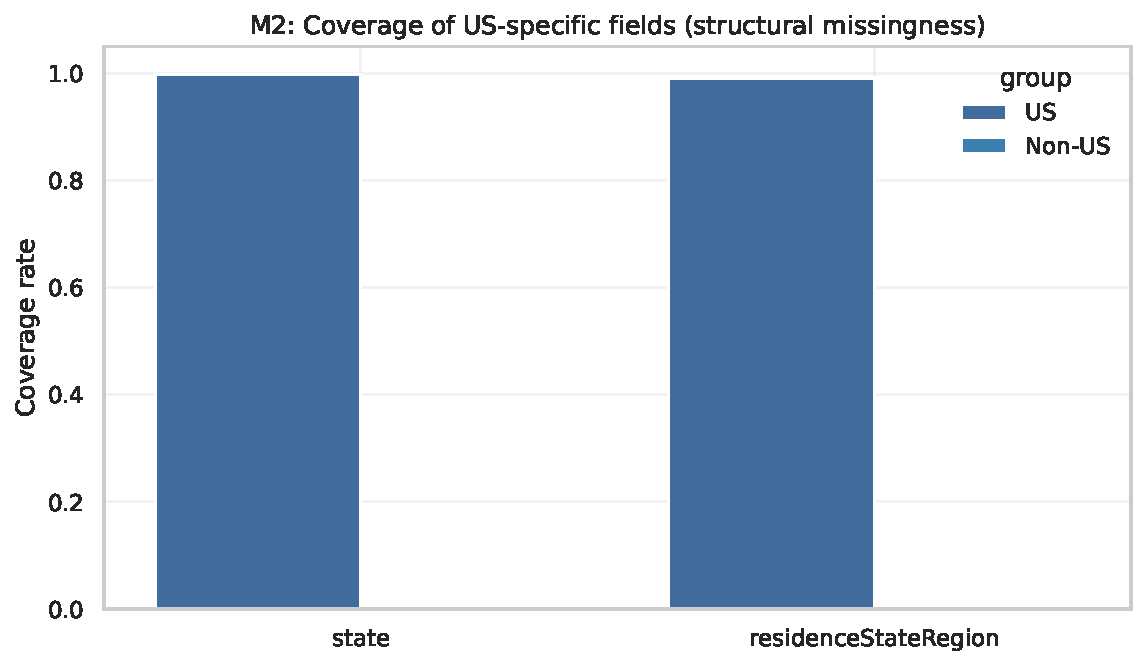
\includegraphics[width=0.88\linewidth]{output/fig/fig_M2_us_only_state_coverage.pdf}
\caption{Structural coverage: U.S.-only population for state/region fields.}
\label{fig:usstate}
\end{figure}

To keep this report honest, we use missingness summaries as a \emph{filter}: variables with structural missingness are either analyzed within the relevant subset (e.g., U.S.\ only) or excluded from global models.
Figure~\ref{fig:miss15} shows overall missingness, and Figure~\ref{fig:missheat} reveals missingness structure by country (top 12 by frequency).

\begin{figure}[H]
\centering
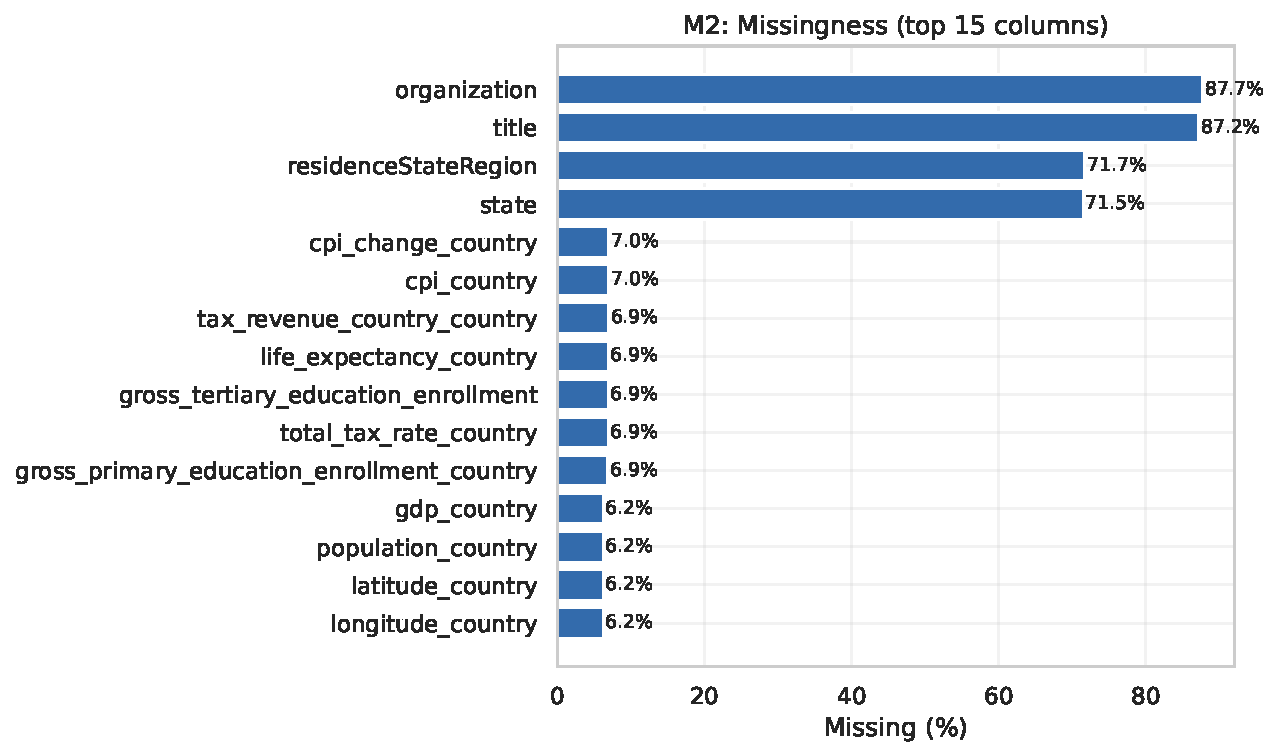
\includegraphics[width=0.86\linewidth]{output/fig/fig_M2_missingness_top15.pdf}
\caption{Top-15 variables by missingness rate.}
\label{fig:miss15}
\end{figure}

\begin{figure}[H]
\centering
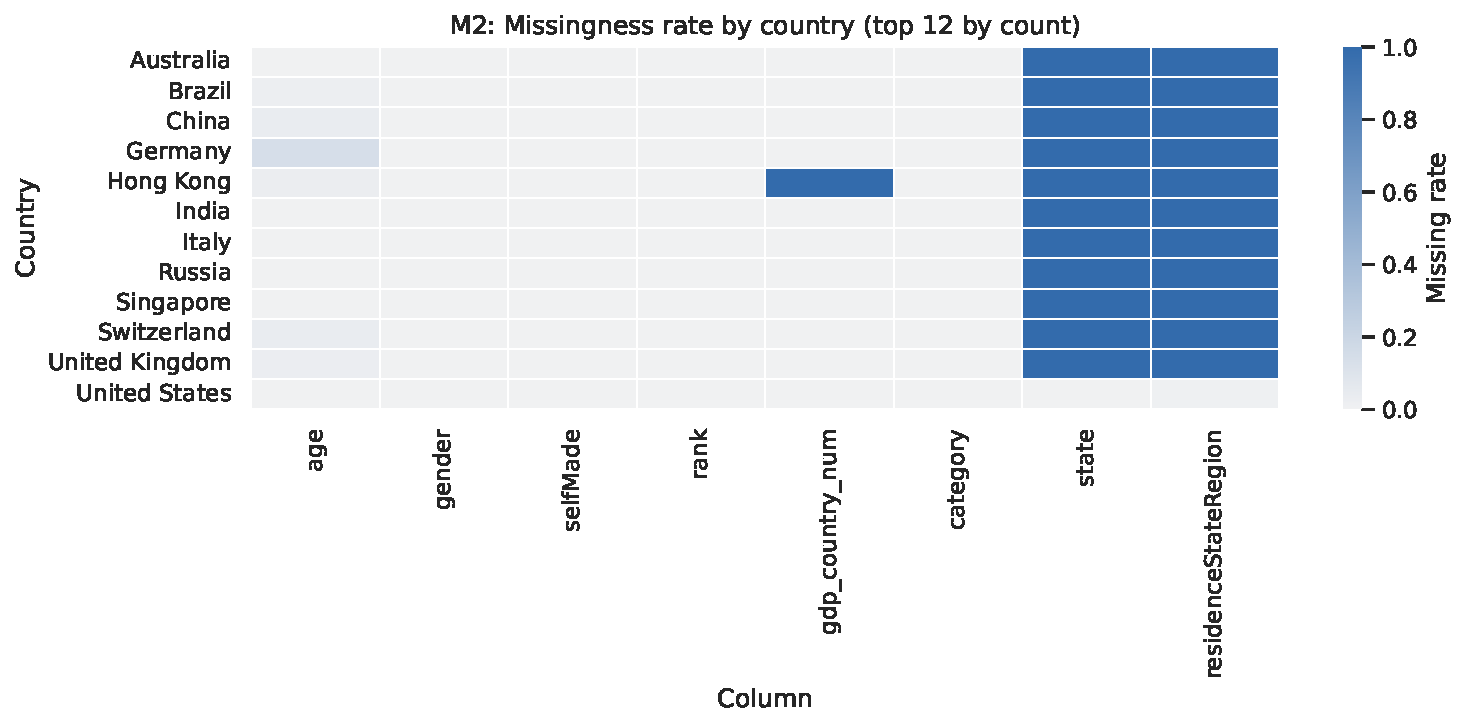
\includegraphics[width=0.92\linewidth]{output/fig/fig_M2_missingness_heatmap_country_top12.pdf}
\caption{Missingness heatmap by country (top 12 by frequency).}
\label{fig:missheat}
\end{figure}

\paragraph{Heavy tails and why we log-transform.}
On the raw scale, billionaire wealth is so skewed that a small number of extreme observations can dominate summaries and models.
We therefore work on the log scale for robustness and interpretability:
\[
\mathrm{log\_finalWorth}=\log\!\bigl(1+\mathrm{finalWorth}\bigr),\qquad
\mathrm{log\_gdp}=\log\!\bigl(1+\mathrm{gdp\_country\_num}\bigr).
\]
Figure~\ref{fig:outlierlog} illustrates why this matters by contrasting raw-scale and log-scale variability.

\begin{figure}[H]
\centering
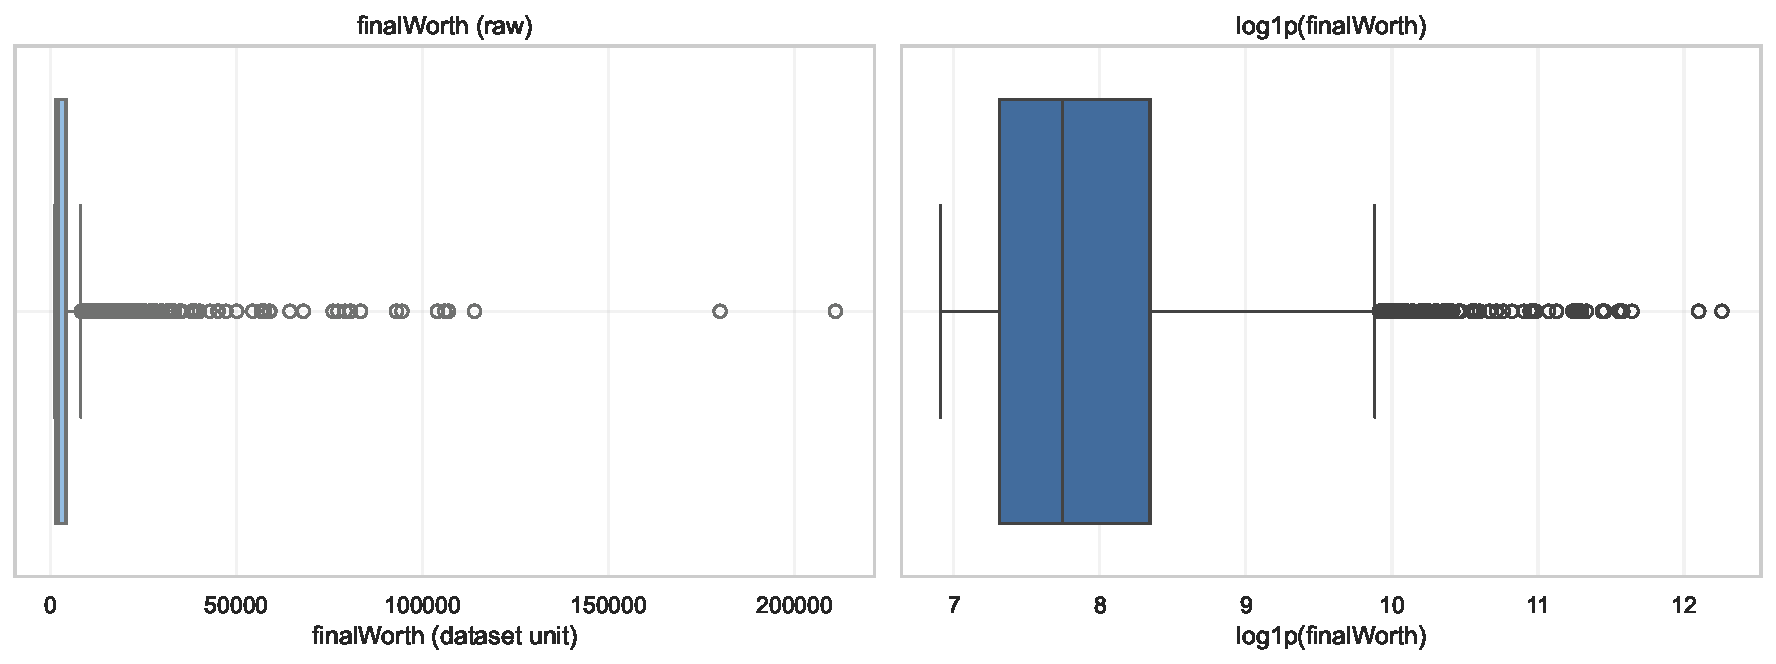
\includegraphics[width=0.84\linewidth]{output/fig/fig_M2_outliers_raw_vs_log_box.pdf}
\caption{Outliers on raw scale vs.\ log scale (heavy-tailed behavior).}
\label{fig:outlierlog}
\end{figure}

\subsection{Descriptive Statistics}\label{sec:desc}

\paragraph{A distribution you should not summarize with ``the average''.}
Figure~\ref{fig:dist} shows the distribution of billionaire wealth on both raw and log scales.
On the raw scale, the plot is dominated by the upper tail; on the log scale, structure becomes visible.
Table~\ref{tab:desc} reports summary statistics that we use throughout the report.

\begin{figure}[H]
\centering
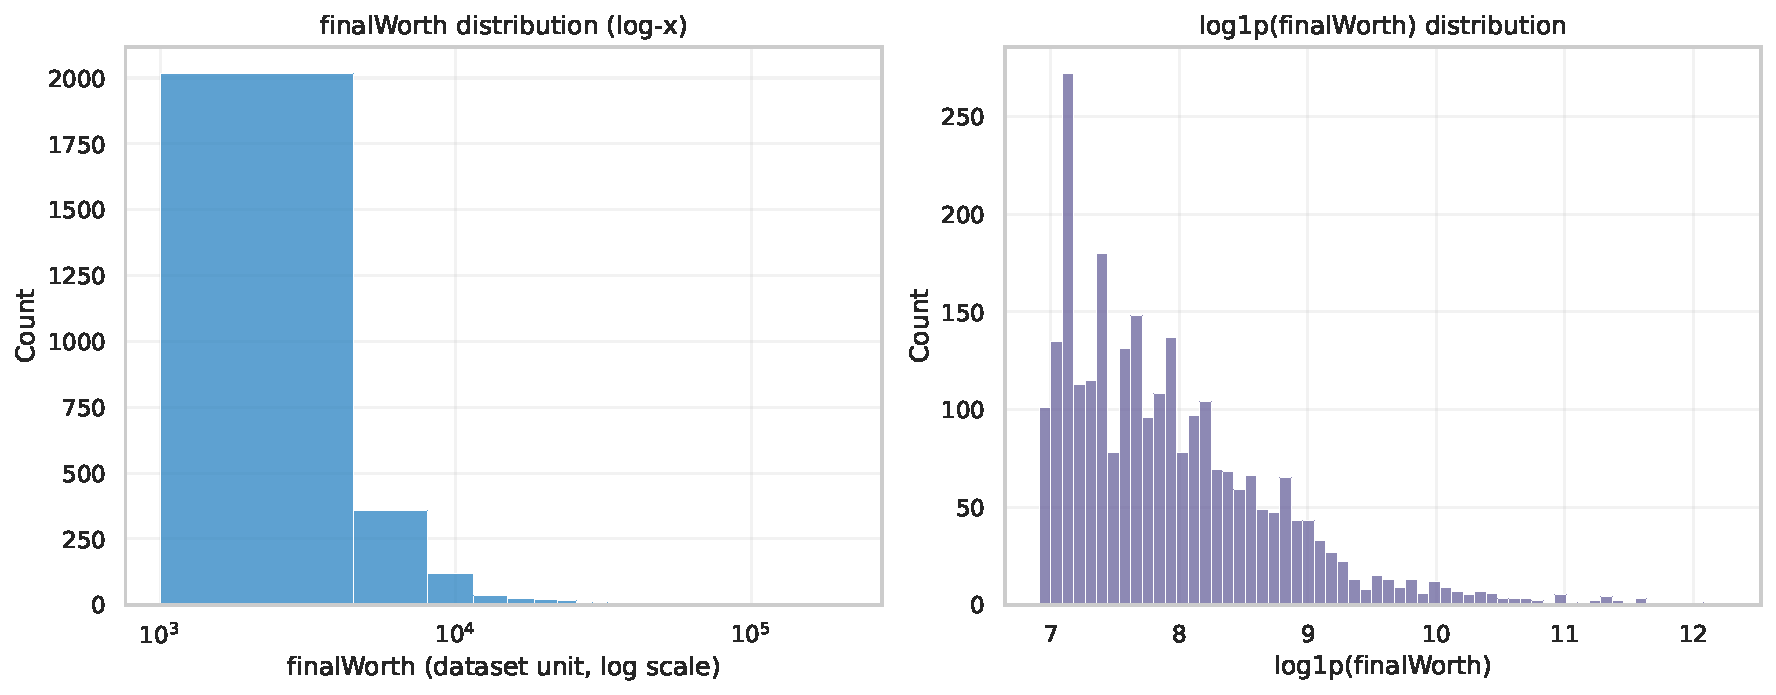
\includegraphics[width=0.90\linewidth]{output/fig/fig_M4_finalWorth_distribution_raw_and_log.pdf}
\caption{Distribution of \texttt{finalWorth} on raw and log scales.}
\label{fig:dist}
\end{figure}

\begin{table}[H]
\centering
\caption{Descriptive statistics for \texttt{finalWorth}.}
\label{tab:desc}
\small
\begin{tabular}{lrr}
\toprule
stat & finalWorth & log1p(finalWorth) \\
\midrule
1\% & 1000.000000 & 6.908755 \\
10\% & 1200.000000 & 7.090910 \\
25\% & 1500.000000 & 7.313887 \\
5\% & 1100.000000 & 7.003974 \\
50\% & 2300.000000 & 7.741099 \\
75\% & 4200.000000 & 8.343078 \\
90\% & 8000.000000 & 8.987322 \\
95\% & 13320.000000 & 9.497076 \\
99\% & 41808.000000 & 10.640328 \\
count & 2640.000000 & 2640.000000 \\
max & 211000.000000 & 12.259618 \\
mean & 4623.787879 & 7.930881 \\
min & 1000.000000 & 6.908755 \\
std & 9834.240939 & 0.820638 \\
\bottomrule
\end{tabular}

\end{table}

\paragraph{Concentration and tail behavior.}
To visualize tail behavior we use the complementary CDF (CCDF). On a log-log scale, the CCDF highlights the heavy tail without forcing a single parametric distributional assumption.
Figure~\ref{fig:ccdf} provides this view.
As a simple concentration summary, we also compute the wealth share held by the top 1\% of records (Figure~\ref{fig:top1}, Table~\ref{tab:top1}).

\begin{figure}[H]
\centering
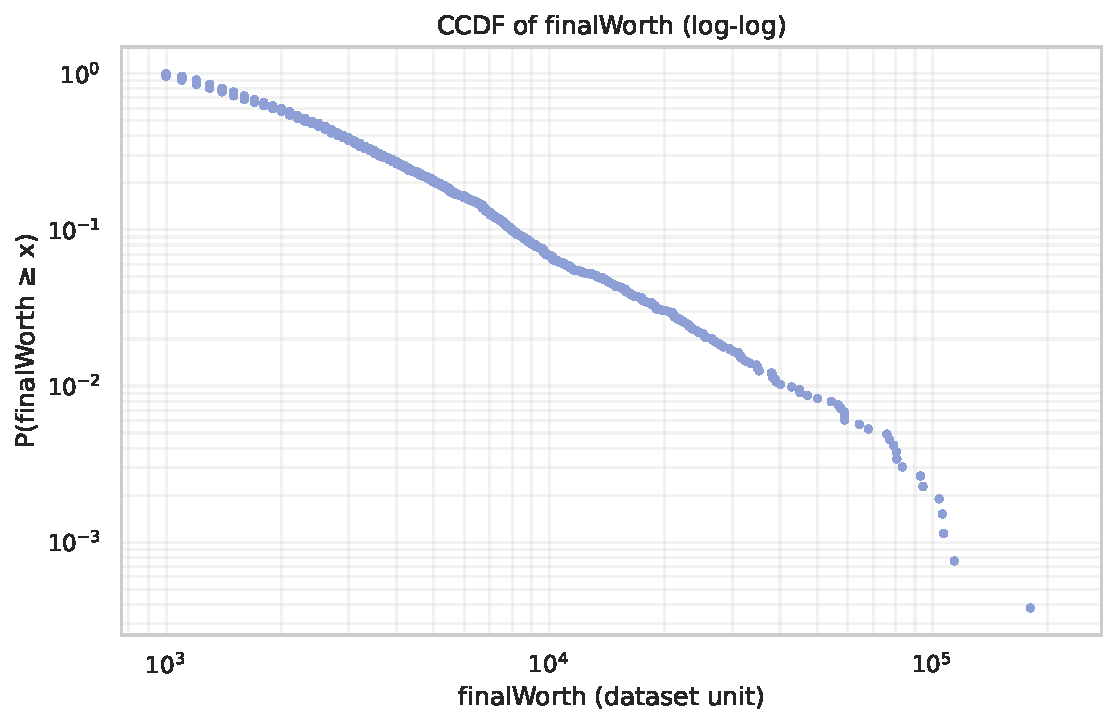
\includegraphics[width=0.88\linewidth]{output/fig/fig_M4_finalWorth_ccdf_loglog.pdf}
\caption{CCDF on log-log scale (heavy-tail visualization).}
\label{fig:ccdf}
\end{figure}

\begin{figure}[H]
\centering
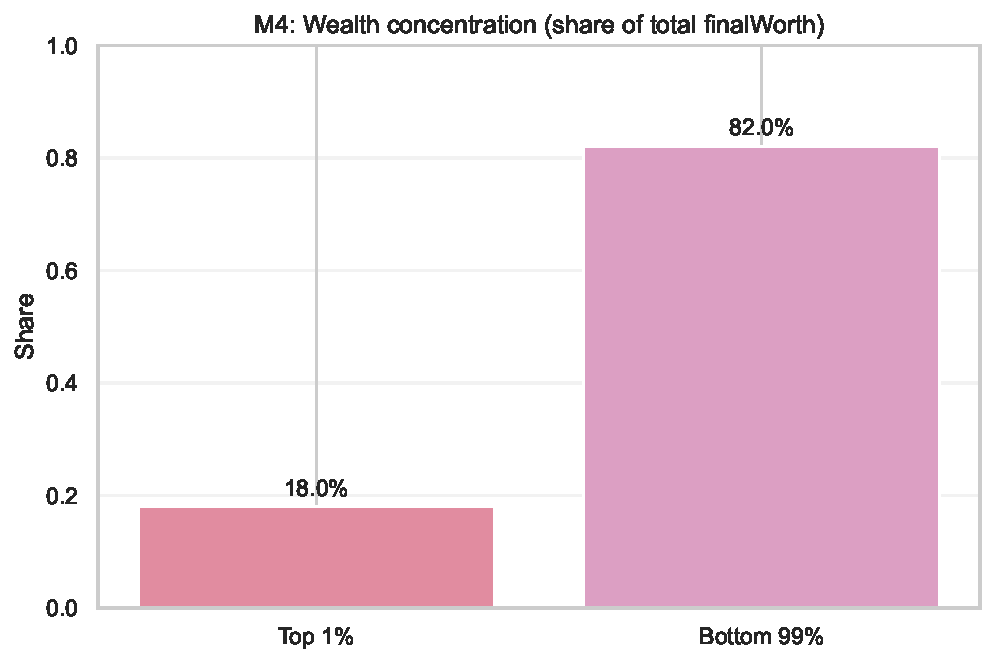
\includegraphics[width=0.78\linewidth]{output/fig/fig_M4_top1pct_wealth_share.pdf}
\caption{Wealth share of the top 1\% of records.}
\label{fig:top1}
\end{figure}

\begin{table}[H]
\centering
\caption{Top-1\% wealth share (numeric summary).}
\label{tab:top1}
\small
\begin{tabular}{rrrr}
\toprule
n\_total & top\_1pct\_n & top\_1pct\_wealth\_share & bottom\_99pct\_wealth\_share \\
\midrule
2640 & 27 & 0.179801 & 0.820199 \\
\bottomrule
\end{tabular}

\end{table}

\paragraph{Where and in what industries?}
Finally, we summarize composition by \texttt{country} and \texttt{category}.
These charts are descriptive---they reflect what is recorded in the dataset, not the true global population of billionaires.
Figures~\ref{fig:topcountry}--\ref{fig:topcat} show the top-10 counts.

\begin{figure}[H]
\centering
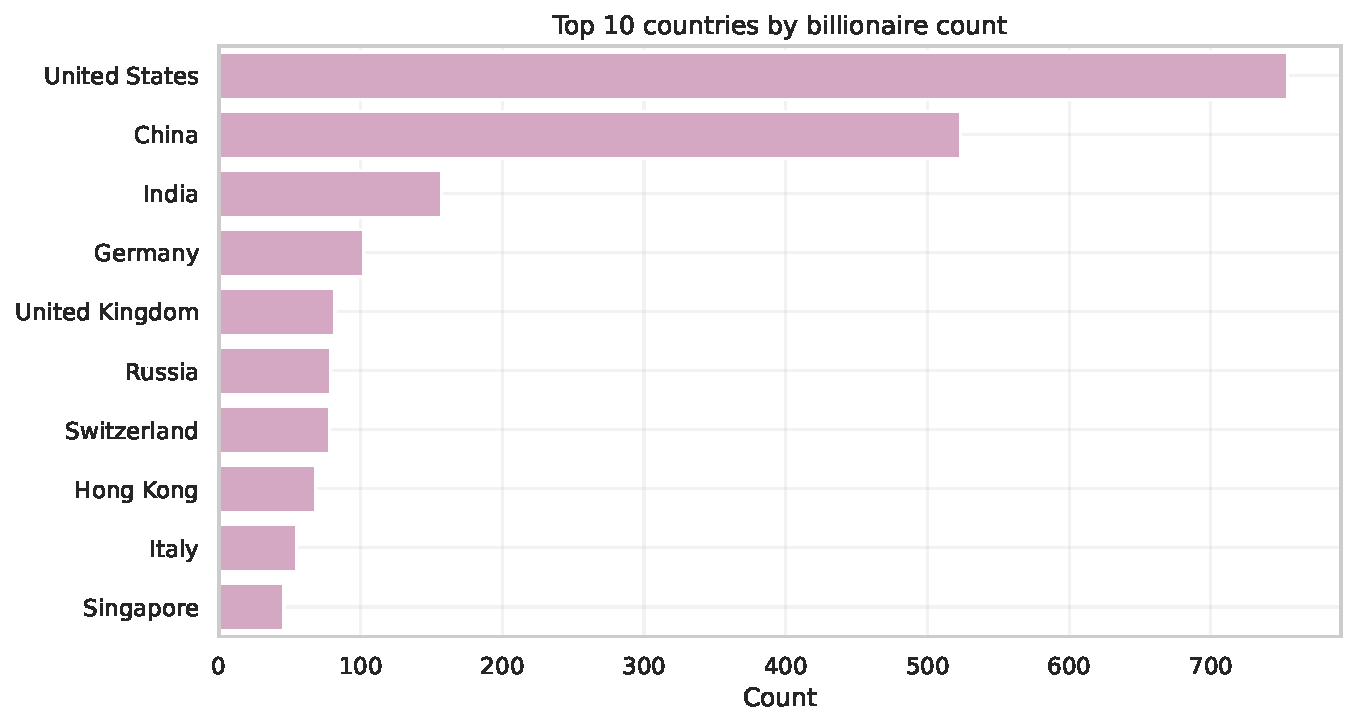
\includegraphics[width=0.82\linewidth]{output/fig/fig_M4_top10_country_count.pdf}
\caption{Top-10 countries by billionaire count.}
\label{fig:topcountry}
\end{figure}

\begin{figure}[H]
\centering
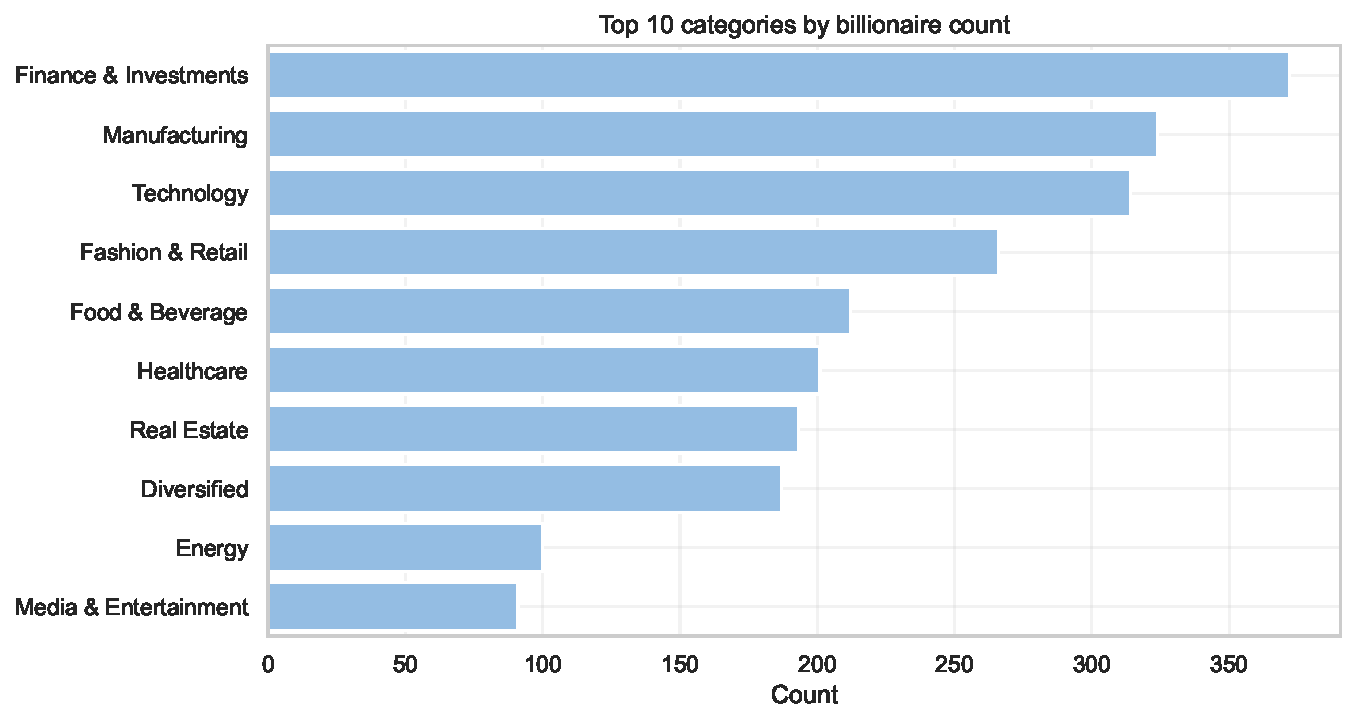
\includegraphics[width=0.82\linewidth]{output/fig/fig_M4_top10_category_count.pdf}
\caption{Top-10 categories by billionaire count.}
\label{fig:topcat}
\end{figure}

\subsection{Inferential Statistics}\label{sec:inf}

\paragraph{Why effect sizes (with CIs) are the main object.}
With thousands of observations, very small differences can be statistically significant.
To avoid ``p-value storytelling'', we report effect sizes with 95\% confidence intervals and include a practical insignificance band in Figure~\ref{fig:forest}.
For two-group comparisons, we use:
mean difference $\Delta=\bar x_1-\bar x_0$,
Cohen's $d$ (standardized mean difference), and Cliff's $\delta$ (stochastic dominance).

For completeness, key definitions are:
\[
r=\frac{\sum_i (x_i-\bar x)(y_i-\bar y)}{\sqrt{\sum_i (x_i-\bar x)^2}\sqrt{\sum_i (y_i-\bar y)^2}},
\qquad
d=\frac{\bar x_1-\bar x_0}{s_p},\ \ 
s_p=\sqrt{\frac{(n_1-1)s_1^2+(n_0-1)s_0^2}{n_1+n_0-2}},
\]
and
\[
\delta = P(X_1>X_0)-P(X_1<X_0).
\]
We compute 95\% bootstrap percentile confidence intervals
\[
\mathrm{CI}_{0.95}=\bigl[Q_{0.025}(\hat\theta^\ast),\, Q_{0.975}(\hat\theta^\ast)\bigr],
\]
where $\hat\theta^\ast$ denotes bootstrap replicates.

Table~\ref{tab:infer} reports correlation estimates and group comparisons, and Figure~\ref{fig:forest} summarizes selected headline effects.

\begin{table}[H]
\centering
\caption{Inferential results with effect sizes and 95\% bootstrap CIs.}
\label{tab:infer}
\small
\begin{tabular}{llrrrrr}
\toprule
family & analysis & n & effect & ci\_low & ci\_high & p\_value \\
\midrule
Correlation & Pearson r (logWorth, logGDP) & 2476 & 0.045759 & 0.007066 & 0.082935 & 0.022786 \\
Correlation & Spearman $\rho$ (logWorth, logGDP) & 2476 & 0.096573 & 0.057546 & 0.136319 & 0.000001 \\
Two-group & Welch t-test: selfMade vs not (logWorth) & 2640 & -0.097502 & -0.168643 & -0.031732 & 0.004980 \\
Two-group & Cohen's d: selfMade vs not (logWorth) & 2640 & -0.118971 & -0.201232 & -0.034527 & 0.004980 \\
Two-group & Cliff's delta: selfMade vs not (logWorth) & 2640 & -0.079194 & -0.124112 & -0.031179 & 0.001072 \\
Robustness & Permutation p-value (mean diff, logWorth) & 2640 & NaN & NaN & NaN & 0.004998 \\
Multi-group & Kruskal-Wallis: logWorth across category & 2640 & 0.008831 & NaN & NaN & 0.001030 \\
\bottomrule
\end{tabular}

\end{table}

\begin{figure}[H]
\centering
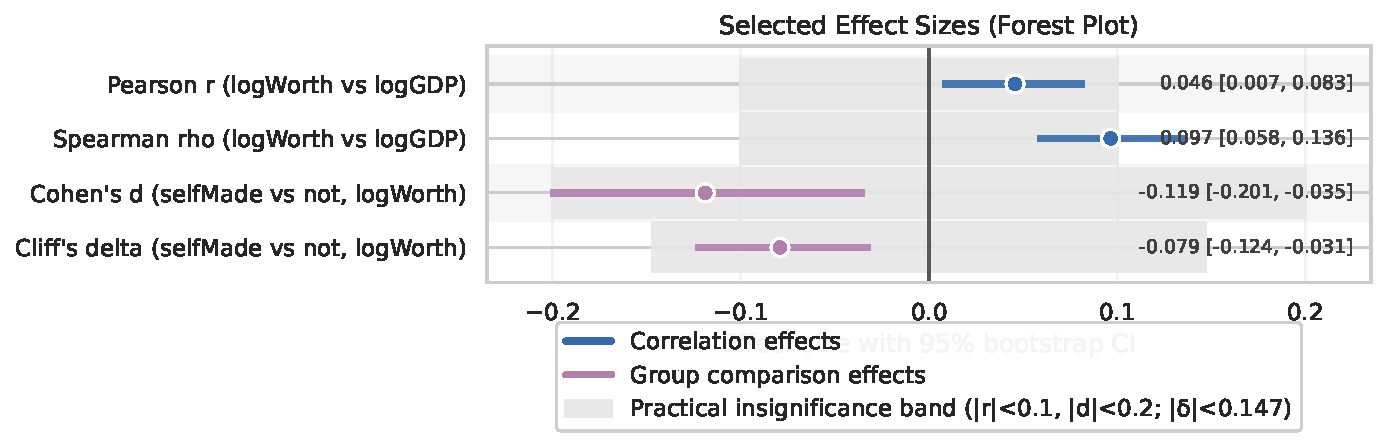
\includegraphics[width=0.92\linewidth]{output/fig/fig_M6_effectsize_forest.pdf}
\caption{Selected effect sizes with 95\% bootstrap confidence intervals. Gray bands indicate ``practically small'' effects (e.g., $|r|<0.1$, $|d|<0.2$).}
\label{fig:forest}
\end{figure}

\subsection{Regression Analysis}\label{sec:reg}

\paragraph{Model specification (association only).}
We fit OLS models to quantify the association between wealth and GDP.
On the log scale:
\[
\mathrm{log\_finalWorth}_i=\beta_0+\beta_1\,\mathrm{log\_gdp}_i+\varepsilon_i.
\]
Interpreting $\beta_1$ as ``elasticity-like'' is convenient (a change in log-wealth per unit change in log-GDP), but it is not a causal effect.

\paragraph{Robust inference and model checking.}
Given heavy tails and likely heteroskedasticity, we report HC3 robust standard errors and 95\% confidence intervals.
Regression coefficients are summarized in Table~\ref{tab:regmain}.
Figure~\ref{fig:regfit} visualizes the fitted association, and Figure~\ref{fig:regdiag} provides basic diagnostics.
We include the Breusch--Pagan test as a heteroskedasticity diagnostic (Table~\ref{tab:bp}).

\begin{table}[H]
\centering
\caption{Regression results (OLS with HC3 robust SE and 95\% CI).}
\label{tab:regmain}
\small
\begin{tabular}{llrrrrrrrr}
\toprule
model & term & coef & se\_hc3 & t & p & ci\_low & ci\_high & n & r2 \\
\midrule
A: finalWorth \textasciitilde \space gdp\_country\_num (HC3) & const & 4237.583714 & 281.536968 & 15.051607 & 0.000000 & 3685.511306 & 4789.656122 & 2476 & 0.001413 \\
A: finalWorth \textasciitilde \space gdp\_country\_num (HC3) & gdp\_country\_num & 0.000000 & 0.000000 & 1.873986 & 0.061050 & -0.000000 & 0.000000 & 2476 & 0.001413 \\
B: log\_finalWorth \textasciitilde \space log\_gdp (HC3) & const & 7.266857 & 0.283538 & 25.629224 & 0.000000 & 6.710861 & 7.822853 & 2476 & 0.002094 \\
B: log\_finalWorth \textasciitilde \space log\_gdp (HC3) & log\_gdp & 0.022871 & 0.009707 & 2.356078 & 0.018547 & 0.003836 & 0.041906 & 2476 & 0.002094 \\
C: log\_finalWorth \textasciitilde \space log\_gdp + controls + C(category) (HC3) & Intercept & 6.387722 & 0.350104 & 18.245205 & 0.000000 & 5.701089 & 7.074355 & 1895 & 0.048394 \\
C: log\_finalWorth \textasciitilde \space log\_gdp + controls + C(category) (HC3) & C(category)[T.Fashion \& Retail] & 0.157747 & 0.086165 & 1.830751 & 0.067296 & -0.011242 & 0.326736 & 1895 & 0.048394 \\
C: log\_finalWorth \textasciitilde \space log\_gdp + controls + C(category) (HC3) & C(category)[T.Finance \& Investments] & 0.118336 & 0.077501 & 1.526885 & 0.126958 & -0.033662 & 0.270333 & 1895 & 0.048394 \\
C: log\_finalWorth \textasciitilde \space log\_gdp + controls + C(category) (HC3) & C(category)[T.Food \& Beverage] & 0.076832 & 0.089285 & 0.860524 & 0.389610 & -0.098276 & 0.251940 & 1895 & 0.048394 \\
C: log\_finalWorth \textasciitilde \space log\_gdp + controls + C(category) (HC3) & C(category)[T.Healthcare] & -0.096619 & 0.081598 & -1.184085 & 0.236529 & -0.256652 & 0.063413 & 1895 & 0.048394 \\
C: log\_finalWorth \textasciitilde \space log\_gdp + controls + C(category) (HC3) & C(category)[T.Manufacturing] & -0.097177 & 0.077834 & -1.248527 & 0.211993 & -0.249826 & 0.055472 & 1895 & 0.048394 \\
C: log\_finalWorth \textasciitilde \space log\_gdp + controls + C(category) (HC3) & C(category)[T.Real Estate] & -0.085950 & 0.080119 & -1.072780 & 0.283507 & -0.243081 & 0.071181 & 1895 & 0.048394 \\
C: log\_finalWorth \textasciitilde \space log\_gdp + controls + C(category) (HC3) & C(category)[T.Technology] & 0.207634 & 0.086833 & 2.391176 & 0.016892 & 0.037334 & 0.377933 & 1895 & 0.048394 \\
C: log\_finalWorth \textasciitilde \space log\_gdp + controls + C(category) (HC3) & log\_gdp & 0.035423 & 0.011781 & 3.006664 & 0.002676 & 0.012317 & 0.058529 & 1895 & 0.048394 \\
C: log\_finalWorth \textasciitilde \space log\_gdp + controls + C(category) (HC3) & age & 0.009192 & 0.001517 & 6.059496 & 0.000000 & 0.006217 & 0.012167 & 1895 & 0.048394 \\
C: log\_finalWorth \textasciitilde \space log\_gdp + controls + C(category) (HC3) & selfMade\_bin & -0.192678 & 0.044844 & -4.296675 & 0.000018 & -0.280627 & -0.104730 & 1895 & 0.048394 \\
C: log\_finalWorth \textasciitilde \space log\_gdp + controls + C(category) (HC3) & gender\_F & -0.040499 & 0.059107 & -0.685179 & 0.493315 & -0.156422 & 0.075424 & 1895 & 0.048394 \\
\bottomrule
\end{tabular}

\end{table}

\begin{figure}[H]
\centering
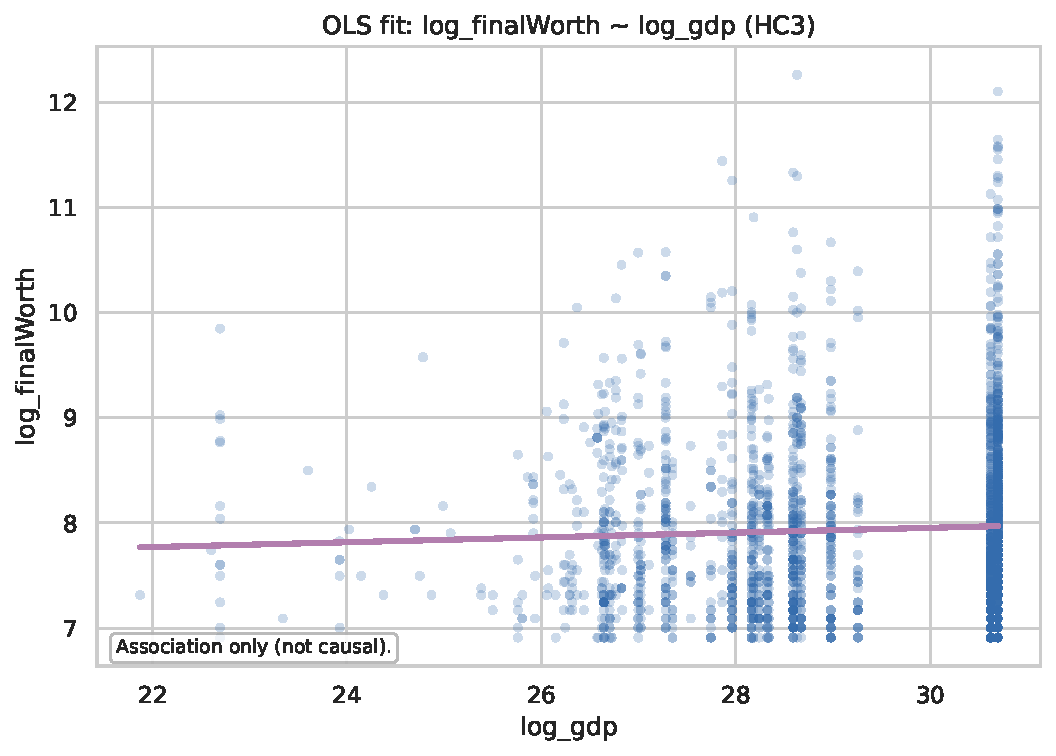
\includegraphics[width=0.86\linewidth]{output/fig/fig_M7_regression_fit_loglog.pdf}
\caption{OLS fit for $\mathrm{log\_finalWorth}\sim \mathrm{log\_gdp}$ (association only).}
\label{fig:regfit}
\end{figure}

\begin{figure}[H]
\centering
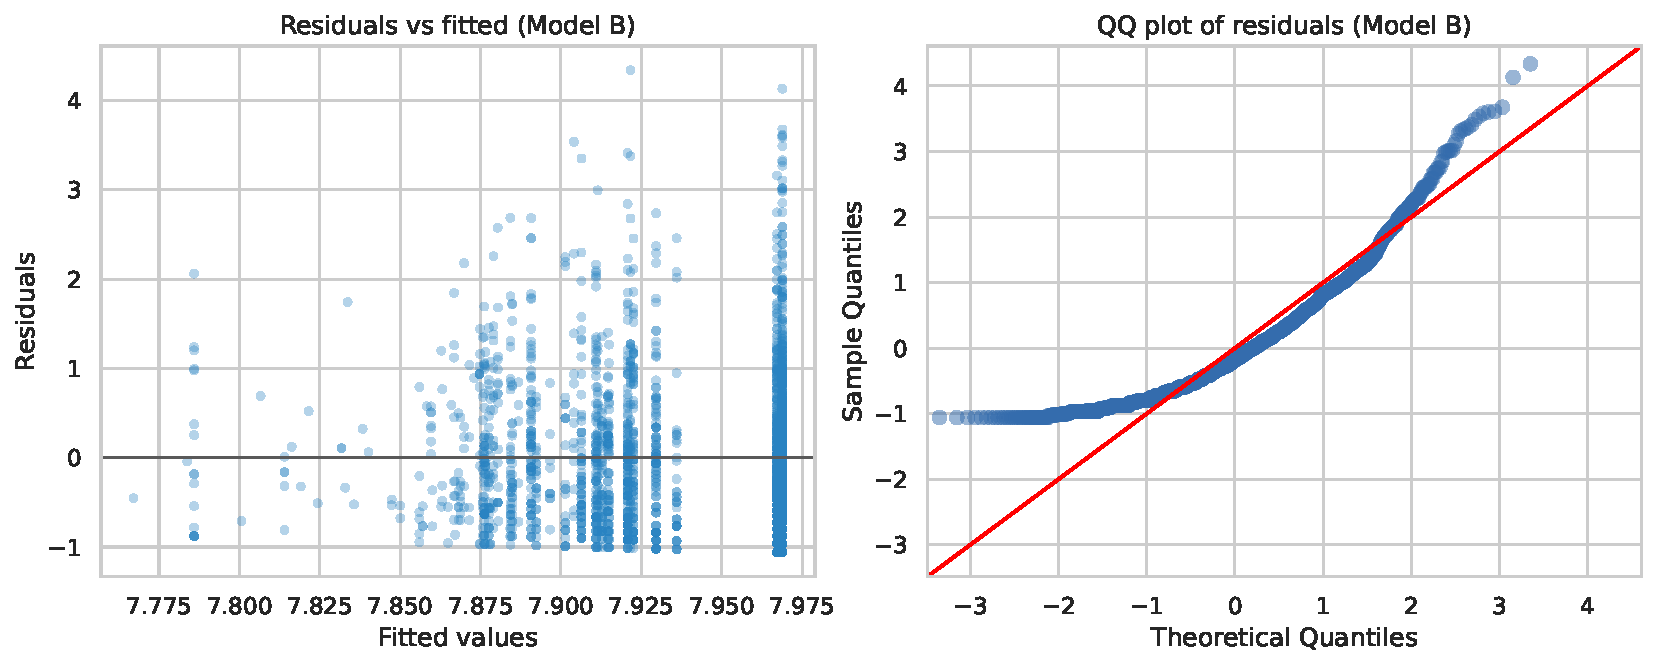
\includegraphics[width=0.92\linewidth]{output/fig/fig_M7_regression_diagnostics.pdf}
\caption{Diagnostics for the main log-log model.}
\label{fig:regdiag}
\end{figure}

\begin{table}[H]
\centering
\caption{Breusch--Pagan test for heteroskedasticity (Model B residuals).}
\label{tab:bp}
\small
\begin{tabular}{rrrrl}
\toprule
lm\_stat & lm\_pvalue & f\_stat & f\_pvalue & note \\
\midrule
2.221610 & 0.136091 & 2.221809 & 0.136201 & Breusch–Pagan test for heteroskedasticity (Model B residuals) \\
\bottomrule
\end{tabular}

\end{table}

\paragraph{Robustness: does the result survive when we remove the extreme tail?}
A fair critique is that the estimated association could be driven by a tiny number of the largest fortunes.
We therefore re-fit the key log model after dropping the top 1\% by \texttt{finalWorth}.
Table~\ref{tab:robtab} and Figure~\ref{fig:robfig} show the stability of $\beta_1$ under this stress test.

\begin{table}[H]
\centering
\caption{Robustness: coefficient on \texttt{log\_gdp} with and without top-1\% exclusion.}
\label{tab:robtab}
\small
\begin{tabular}{lrrrr}
\toprule
setting & n & coef\_log\_gdp & ci\_low & ci\_high \\
\midrule
All complete cases & 2476 & 0.022871 & 0.003836 & 0.041906 \\
Drop top 1\% finalWorth & 2451 & 0.013569 & -0.004519 & 0.031658 \\
\bottomrule
\end{tabular}

\end{table}

\begin{figure}[H]
\centering
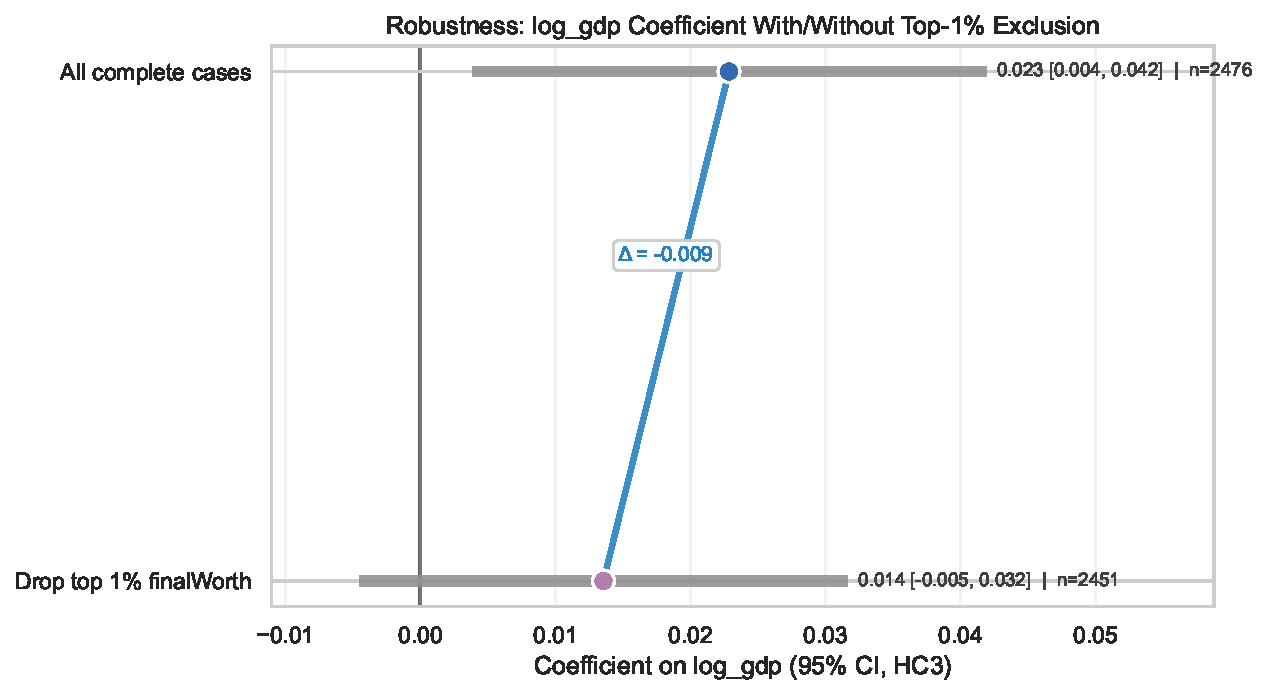
\includegraphics[width=0.88\linewidth]{output/fig/fig_M7_robust_coef_compare_top1pct.pdf}
\caption{Robustness: connected dumbbell comparison of $\beta_1$ across settings (95\% CI).}
\label{fig:robfig}
\end{figure}

\section{Key Insights and Limitations}\label{sec:insights}

This section presents the story in its final form: four takeaways (two core, two exploratory), each tied to concrete evidence and at least one robustness consideration.

\subsection{Core Insight 1: Billionaire wealth is dominated by the upper tail}

The dataset behaves like many ``extreme outcome'' datasets: the main challenge is not estimating the center, but understanding the tail.
On the raw scale (Figure~\ref{fig:dist}), a handful of observations visually dominate the distribution; on the log scale, the rest of the data becomes visible.
The CCDF (Figure~\ref{fig:ccdf}) makes the same point from a different angle: the tail decays slowly, so small changes in how we handle extremes can change results.
\textbf{Design response:} we report key results on a log scale and avoid interpreting raw-scale averages as ``typical'' wealth.

\subsection{Core Insight 2: Wealth--GDP association is present but should be read as non-causal}

Across countries in this dataset, higher GDP is associated with higher recorded billionaire wealth.
The regression table (Table~\ref{tab:regmain}) and fitted plot (Figure~\ref{fig:regfit}) summarize this relationship on the log scale.
However, this is an observational association: GDP may proxy institutions, market size, reporting intensity, and historical accumulation.
\textbf{Design response:} inference uses HC3 robust SE, diagnostics are reported (Figure~\ref{fig:regdiag}, Table~\ref{tab:bp}), and we stress-test the key coefficient by excluding the top 1\% of fortunes (Table~\ref{tab:robtab}, Figure~\ref{fig:robfig}).

\subsection{Exploratory Insight 1: Missingness is structured, not random}

A story that ignores missingness can easily become fiction.
Here, the state/region fields are essentially U.S.-only (Figure~\ref{fig:usstate}), which means those variables cannot be treated as universally observed.
Country-dependent missingness patterns also appear in the heatmap (Figure~\ref{fig:missheat}).
\textbf{Design response:} we either restrict those variables to the relevant subset (U.S.\ records) or keep them out of global models, and we interpret cross-country patterns as ``recorded in this dataset'' rather than population truth.

\subsection{Exploratory Insight 2: Effect sizes help separate ``real'' from ``important''}

Because the dataset is large, some effects can be statistically detectable even when practically small.
Figure~\ref{fig:forest} adds a practical insignificance band to keep interpretation grounded (e.g., $|r|<0.1$ and $|d|<0.2$).
Table~\ref{tab:infer} reports the full set of effect sizes with bootstrap CIs, which is more informative than a $p$-value-only summary.
\textbf{Design response:} we discuss effect size magnitudes and uncertainty, not just significance.

\subsection{Limitations}

\begin{itemize}
  \item \textbf{Observational data:} no causal claims are made. GDP is correlated with many unmeasured confounders.
  \item \textbf{Dataset coverage:} the dataset is curated and may reflect reporting/collection practices; composition charts are descriptive of the dataset, not the world.
  \item \textbf{Documentation gaps:} when variable units or definitions are not fully documented, we avoid over-precise interpretations and focus on internally consistent comparisons.
\end{itemize}

\section{References}

\begin{itemize}
  \item Course-provided dataset: \textit{Billionaires Statistics Dataset.csv}.
  \item Python scientific stack: pandas, numpy, scipy, statsmodels, matplotlib (versions recorded in Table~\ref{tab:env}).
\end{itemize}

\appendix
\section{Reproducibility and Notebook Appendix}

\begin{table}[H]
\centering
\caption{Environment snapshot (for reproducibility).}
\label{tab:env}
\small
\begin{tabular}{lllllll}
\toprule
timestamp & python & platform & numpy & pandas & matplotlib & seaborn \\
\midrule
2026-02-28T02:13:50 & 3.13.5 & Windows-11-10.0.26100-SP0 & 2.1.3 & 2.2.3 & 3.10.0 & 0.13.2 \\
\bottomrule
\end{tabular}

\end{table}

\begin{table}[H]
\centering
\caption{Runbook for reproducing all artifacts.}
\label{tab:runbook}
\small
\begin{tabular}{rl}
\toprule
step & action \\
\midrule
1 & Place the raw CSV at ./data/raw/Billionaires Statistics Dataset.csv \\
2 & Open ./supplemental\_code.ipynb \\
3 & Kernel → Restart \& Run All \\
4 & Verify outputs in ./output/fig and ./output/tab \\
5 & Use tab\_M9\_report\_map to reference figures/tables in the report \\
\bottomrule
\end{tabular}

\end{table}

\begin{table}[H]
\centering
\caption{Report map: where each figure/table is used.}
\label{tab:reportmap}
\scriptsize
\begin{tabular}{lllll}
\toprule
report\_section & module & kind & name & paths \\
\midrule
Introduction & M0 & figure & fig\_M0\_variable\_role\_counts & \{"pdf": "/mnt/e/canfiles/Common courses study/\textbackslash u5927\textbackslash u5b66\textbackslash u901a\textbackslash u8bc6/25-26 Spring/UFUG 2104 Applied statistics/final\_project\_v3/output/fig/fig\_M0\_variable\_role\_counts.pdf", "png": "/mnt/e/canfiles/Common courses study/\textbackslash u5927\textbackslash u5b66\textbackslash u901a\textbackslash u8bc6/25-26 Spring/UFUG 2104 Applied statistics/final\_project\_v3/output/fig/fig\_M0\_variable\_role\_counts.png"\} \\
Introduction & M0 & table & tab\_M0\_environment\_snapshot & \{"csv": "/mnt/e/canfiles/Common courses study/\textbackslash u5927\textbackslash u5b66\textbackslash u901a\textbackslash u8bc6/25-26 Spring/UFUG 2104 Applied statistics/final\_project\_v3/output/tab/tab\_M0\_environment\_snapshot.csv", "tex": "/mnt/e/canfiles/Common courses study/\textbackslash u5927\textbackslash u5b66\textbackslash u901a\textbackslash u8bc6/25-26 Spring/UFUG 2104 Applied statistics/final\_project\_v3/output/tab/tab\_M0\_environment\_snapshot.tex"\} \\
Introduction & M0 & table & tab\_M0\_research\_questions & \{"csv": "/mnt/e/canfiles/Common courses study/\textbackslash u5927\textbackslash u5b66\textbackslash u901a\textbackslash u8bc6/25-26 Spring/UFUG 2104 Applied statistics/final\_project\_v3/output/tab/tab\_M0\_research\_questions.csv", "tex": "/mnt/e/canfiles/Common courses study/\textbackslash u5927\textbackslash u5b66\textbackslash u901a\textbackslash u8bc6/25-26 Spring/UFUG 2104 Applied statistics/final\_project\_v3/output/tab/tab\_M0\_research\_questions.tex"\} \\
Introduction & M0 & table & tab\_M0\_research\_questions\_source & \{"csv": "/mnt/e/canfiles/Common courses study/\textbackslash u5927\textbackslash u5b66\textbackslash u901a\textbackslash u8bc6/25-26 Spring/UFUG 2104 Applied statistics/final\_project\_v3/output/tab/tab\_M0\_research\_questions\_source.csv", "tex": "/mnt/e/canfiles/Common courses study/\textbackslash u5927\textbackslash u5b66\textbackslash u901a\textbackslash u8bc6/25-26 Spring/UFUG 2104 Applied statistics/final\_project\_v3/output/tab/tab\_M0\_research\_questions\_source.tex"\} \\
Introduction & M0 & table & tab\_M0\_schema\_freeze\_A\_summary & \{"csv": "/mnt/e/canfiles/Common courses study/\textbackslash u5927\textbackslash u5b66\textbackslash u901a\textbackslash u8bc6/25-26 Spring/UFUG 2104 Applied statistics/final\_project\_v3/output/tab/tab\_M0\_schema\_freeze\_A\_summary.csv", "tex": "/mnt/e/canfiles/Common courses study/\textbackslash u5927\textbackslash u5b66\textbackslash u901a\textbackslash u8bc6/25-26 Spring/UFUG 2104 Applied statistics/final\_project\_v3/output/tab/tab\_M0\_schema\_freeze\_A\_summary.tex"\} \\
Introduction & M0 & table & tab\_M0\_variable\_roles & \{"csv": "/mnt/e/canfiles/Common courses study/\textbackslash u5927\textbackslash u5b66\textbackslash u901a\textbackslash u8bc6/25-26 Spring/UFUG 2104 Applied statistics/final\_project\_v3/output/tab/tab\_M0\_variable\_roles.csv", "tex": "/mnt/e/canfiles/Common courses study/\textbackslash u5927\textbackslash u5b66\textbackslash u901a\textbackslash u8bc6/25-26 Spring/UFUG 2104 Applied statistics/final\_project\_v3/output/tab/tab\_M0\_variable\_roles.tex"\} \\
Introduction (Dataset overview) & M1 & figure & fig\_M1\_dtype\_distribution & \{"pdf": "/mnt/e/canfiles/Common courses study/\textbackslash u5927\textbackslash u5b66\textbackslash u901a\textbackslash u8bc6/25-26 Spring/UFUG 2104 Applied statistics/final\_project\_v3/output/fig/fig\_M1\_dtype\_distribution.pdf", "png": "/mnt/e/canfiles/Common courses study/\textbackslash u5927\textbackslash u5b66\textbackslash u901a\textbackslash u8bc6/25-26 Spring/UFUG 2104 Applied statistics/final\_project\_v3/output/fig/fig\_M1\_dtype\_distribution.png"\} \\
Introduction (Dataset overview) & M1 & table & tab\_M1\_dictionary\_verification\_checks & \{"csv": "/mnt/e/canfiles/Common courses study/\textbackslash u5927\textbackslash u5b66\textbackslash u901a\textbackslash u8bc6/25-26 Spring/UFUG 2104 Applied statistics/final\_project\_v3/output/tab/tab\_M1\_dictionary\_verification\_checks.csv", "tex": "/mnt/e/canfiles/Common courses study/\textbackslash u5927\textbackslash u5b66\textbackslash u901a\textbackslash u8bc6/25-26 Spring/UFUG 2104 Applied statistics/final\_project\_v3/output/tab/tab\_M1\_dictionary\_verification\_checks.tex"\} \\
Introduction (Dataset overview) & M1 & table & tab\_M1\_gdp\_parse\_summary & \{"csv": "/mnt/e/canfiles/Common courses study/\textbackslash u5927\textbackslash u5b66\textbackslash u901a\textbackslash u8bc6/25-26 Spring/UFUG 2104 Applied statistics/final\_project\_v3/output/tab/tab\_M1\_gdp\_parse\_summary.csv", "tex": "/mnt/e/canfiles/Common courses study/\textbackslash u5927\textbackslash u5b66\textbackslash u901a\textbackslash u8bc6/25-26 Spring/UFUG 2104 Applied statistics/final\_project\_v3/output/tab/tab\_M1\_gdp\_parse\_summary.tex"\} \\
Introduction (Dataset overview) & M1 & table & tab\_M1\_schema\_summary & \{"csv": "/mnt/e/canfiles/Common courses study/\textbackslash u5927\textbackslash u5b66\textbackslash u901a\textbackslash u8bc6/25-26 Spring/UFUG 2104 Applied statistics/final\_project\_v3/output/tab/tab\_M1\_schema\_summary.csv", "tex": "/mnt/e/canfiles/Common courses study/\textbackslash u5927\textbackslash u5b66\textbackslash u901a\textbackslash u8bc6/25-26 Spring/UFUG 2104 Applied statistics/final\_project\_v3/output/tab/tab\_M1\_schema\_summary.tex"\} \\
Introduction (Dataset overview) & M1 & table & tab\_M1\_v2\_to\_current\_rq\_coverage & \{"csv": "/mnt/e/canfiles/Common courses study/\textbackslash u5927\textbackslash u5b66\textbackslash u901a\textbackslash u8bc6/25-26 Spring/UFUG 2104 Applied statistics/final\_project\_v3/output/tab/tab\_M1\_v2\_to\_current\_rq\_coverage.csv", "tex": "/mnt/e/canfiles/Common courses study/\textbackslash u5927\textbackslash u5b66\textbackslash u901a\textbackslash u8bc6/25-26 Spring/UFUG 2104 Applied statistics/final\_project\_v3/output/tab/tab\_M1\_v2\_to\_current\_rq\_coverage.tex"\} \\
Introduction (Dataset overview) & M1 & table & tab\_M1\_v2\_topic\_reasoning\_archive & \{"csv": "/mnt/e/canfiles/Common courses study/\textbackslash u5927\textbackslash u5b66\textbackslash u901a\textbackslash u8bc6/25-26 Spring/UFUG 2104 Applied statistics/final\_project\_v3/output/tab/tab\_M1\_v2\_topic\_reasoning\_archive.csv", "tex": "/mnt/e/canfiles/Common courses study/\textbackslash u5927\textbackslash u5b66\textbackslash u901a\textbackslash u8bc6/25-26 Spring/UFUG 2104 Applied statistics/final\_project\_v3/output/tab/tab\_M1\_v2\_topic\_reasoning\_archive.tex"\} \\
Statistical Analysis (Data Quality) & M2 & figure & fig\_M2\_missingness\_heatmap\_country\_top12 & \{"pdf": "/mnt/e/canfiles/Common courses study/\textbackslash u5927\textbackslash u5b66\textbackslash u901a\textbackslash u8bc6/25-26 Spring/UFUG 2104 Applied statistics/final\_project\_v3/output/fig/fig\_M2\_missingness\_heatmap\_country\_top12.pdf", "png": "/mnt/e/canfiles/Common courses study/\textbackslash u5927\textbackslash u5b66\textbackslash u901a\textbackslash u8bc6/25-26 Spring/UFUG 2104 Applied statistics/final\_project\_v3/output/fig/fig\_M2\_missingness\_heatmap\_country\_top12.png"\} \\
Statistical Analysis (Data Quality) & M2 & figure & fig\_M2\_missingness\_top15 & \{"pdf": "/mnt/e/canfiles/Common courses study/\textbackslash u5927\textbackslash u5b66\textbackslash u901a\textbackslash u8bc6/25-26 Spring/UFUG 2104 Applied statistics/final\_project\_v3/output/fig/fig\_M2\_missingness\_top15.pdf", "png": "/mnt/e/canfiles/Common courses study/\textbackslash u5927\textbackslash u5b66\textbackslash u901a\textbackslash u8bc6/25-26 Spring/UFUG 2104 Applied statistics/final\_project\_v3/output/fig/fig\_M2\_missingness\_top15.png"\} \\
Statistical Analysis (Data Quality) & M2 & figure & fig\_M2\_outliers\_raw\_vs\_log\_box & \{"pdf": "/mnt/e/canfiles/Common courses study/\textbackslash u5927\textbackslash u5b66\textbackslash u901a\textbackslash u8bc6/25-26 Spring/UFUG 2104 Applied statistics/final\_project\_v3/output/fig/fig\_M2\_outliers\_raw\_vs\_log\_box.pdf", "png": "/mnt/e/canfiles/Common courses study/\textbackslash u5927\textbackslash u5b66\textbackslash u901a\textbackslash u8bc6/25-26 Spring/UFUG 2104 Applied statistics/final\_project\_v3/output/fig/fig\_M2\_outliers\_raw\_vs\_log\_box.png"\} \\
Statistical Analysis (Data Quality) & M2 & figure & fig\_M2\_us\_only\_state\_coverage & \{"pdf": "/mnt/e/canfiles/Common courses study/\textbackslash u5927\textbackslash u5b66\textbackslash u901a\textbackslash u8bc6/25-26 Spring/UFUG 2104 Applied statistics/final\_project\_v3/output/fig/fig\_M2\_us\_only\_state\_coverage.pdf", "png": "/mnt/e/canfiles/Common courses study/\textbackslash u5927\textbackslash u5b66\textbackslash u901a\textbackslash u8bc6/25-26 Spring/UFUG 2104 Applied statistics/final\_project\_v3/output/fig/fig\_M2\_us\_only\_state\_coverage.png"\} \\
Statistical Analysis (Data Quality) & M2 & table & tab\_M2\_artifact\_index & \{"csv": "/mnt/e/canfiles/Common courses study/\textbackslash u5927\textbackslash u5b66\textbackslash u901a\textbackslash u8bc6/25-26 Spring/UFUG 2104 Applied statistics/final\_project\_v3/output/tab/tab\_M2\_artifact\_index.csv", "tex": "/mnt/e/canfiles/Common courses study/\textbackslash u5927\textbackslash u5b66\textbackslash u901a\textbackslash u8bc6/25-26 Spring/UFUG 2104 Applied statistics/final\_project\_v3/output/tab/tab\_M2\_artifact\_index.tex"\} \\
Statistical Analysis (Data Quality) & M2 & table & tab\_M2\_dq\_issues\_summary & \{"csv": "/mnt/e/canfiles/Common courses study/\textbackslash u5927\textbackslash u5b66\textbackslash u901a\textbackslash u8bc6/25-26 Spring/UFUG 2104 Applied statistics/final\_project\_v3/output/tab/tab\_M2\_dq\_issues\_summary.csv", "tex": "/mnt/e/canfiles/Common courses study/\textbackslash u5927\textbackslash u5b66\textbackslash u901a\textbackslash u8bc6/25-26 Spring/UFUG 2104 Applied statistics/final\_project\_v3/output/tab/tab\_M2\_dq\_issues\_summary.tex"\} \\
Statistical Analysis (Data Quality) & M2 & table & tab\_M2\_missingness\_by\_country\_top12 & \{"csv": "/mnt/e/canfiles/Common courses study/\textbackslash u5927\textbackslash u5b66\textbackslash u901a\textbackslash u8bc6/25-26 Spring/UFUG 2104 Applied statistics/final\_project\_v3/output/tab/tab\_M2\_missingness\_by\_country\_top12.csv", "tex": "/mnt/e/canfiles/Common courses study/\textbackslash u5927\textbackslash u5b66\textbackslash u901a\textbackslash u8bc6/25-26 Spring/UFUG 2104 Applied statistics/final\_project\_v3/output/tab/tab\_M2\_missingness\_by\_country\_top12.tex"\} \\
Statistical Analysis (Data Quality) & M2 & table & tab\_M2\_missingness\_top15 & \{"csv": "/mnt/e/canfiles/Common courses study/\textbackslash u5927\textbackslash u5b66\textbackslash u901a\textbackslash u8bc6/25-26 Spring/UFUG 2104 Applied statistics/final\_project\_v3/output/tab/tab\_M2\_missingness\_top15.csv", "tex": "/mnt/e/canfiles/Common courses study/\textbackslash u5927\textbackslash u5b66\textbackslash u901a\textbackslash u8bc6/25-26 Spring/UFUG 2104 Applied statistics/final\_project\_v3/output/tab/tab\_M2\_missingness\_top15.tex"\} \\
Statistical Analysis (Data Quality) & M2 & table & tab\_M2\_us\_only\_state\_coverage & \{"csv": "/mnt/e/canfiles/Common courses study/\textbackslash u5927\textbackslash u5b66\textbackslash u901a\textbackslash u8bc6/25-26 Spring/UFUG 2104 Applied statistics/final\_project\_v3/output/tab/tab\_M2\_us\_only\_state\_coverage.csv", "tex": "/mnt/e/canfiles/Common courses study/\textbackslash u5927\textbackslash u5b66\textbackslash u901a\textbackslash u8bc6/25-26 Spring/UFUG 2104 Applied statistics/final\_project\_v3/output/tab/tab\_M2\_us\_only\_state\_coverage.tex"\} \\
Statistical Analysis (Cleaning) & M3 & figure & fig\_M3\_validation\_log\_distributions & \{"pdf": "/mnt/e/canfiles/Common courses study/\textbackslash u5927\textbackslash u5b66\textbackslash u901a\textbackslash u8bc6/25-26 Spring/UFUG 2104 Applied statistics/final\_project\_v3/output/fig/fig\_M3\_validation\_log\_distributions.pdf", "png": "/mnt/e/canfiles/Common courses study/\textbackslash u5927\textbackslash u5b66\textbackslash u901a\textbackslash u8bc6/25-26 Spring/UFUG 2104 Applied statistics/final\_project\_v3/output/fig/fig\_M3\_validation\_log\_distributions.png"\} \\
Statistical Analysis (Cleaning) & M3 & table & tab\_M3\_clean\_dataset\_manifest & \{"csv": "/mnt/e/canfiles/Common courses study/\textbackslash u5927\textbackslash u5b66\textbackslash u901a\textbackslash u8bc6/25-26 Spring/UFUG 2104 Applied statistics/final\_project\_v3/output/tab/tab\_M3\_clean\_dataset\_manifest.csv", "tex": "/mnt/e/canfiles/Common courses study/\textbackslash u5927\textbackslash u5b66\textbackslash u901a\textbackslash u8bc6/25-26 Spring/UFUG 2104 Applied statistics/final\_project\_v3/output/tab/tab\_M3\_clean\_dataset\_manifest.tex"\} \\
Statistical Analysis (Cleaning) & M3 & table & tab\_M3\_cleaning\_log & \{"csv": "/mnt/e/canfiles/Common courses study/\textbackslash u5927\textbackslash u5b66\textbackslash u901a\textbackslash u8bc6/25-26 Spring/UFUG 2104 Applied statistics/final\_project\_v3/output/tab/tab\_M3\_cleaning\_log.csv", "tex": "/mnt/e/canfiles/Common courses study/\textbackslash u5927\textbackslash u5b66\textbackslash u901a\textbackslash u8bc6/25-26 Spring/UFUG 2104 Applied statistics/final\_project\_v3/output/tab/tab\_M3\_cleaning\_log.tex"\} \\
Statistical Analysis (Descriptive) & M4 & figure & fig\_M4\_finalWorth\_ccdf\_loglog & \{"pdf": "/mnt/e/canfiles/Common courses study/\textbackslash u5927\textbackslash u5b66\textbackslash u901a\textbackslash u8bc6/25-26 Spring/UFUG 2104 Applied statistics/final\_project\_v3/output/fig/fig\_M4\_finalWorth\_ccdf\_loglog.pdf", "png": "/mnt/e/canfiles/Common courses study/\textbackslash u5927\textbackslash u5b66\textbackslash u901a\textbackslash u8bc6/25-26 Spring/UFUG 2104 Applied statistics/final\_project\_v3/output/fig/fig\_M4\_finalWorth\_ccdf\_loglog.png"\} \\
Statistical Analysis (Descriptive) & M4 & figure & fig\_M4\_finalWorth\_distribution\_raw\_and\_log & \{"pdf": "/mnt/e/canfiles/Common courses study/\textbackslash u5927\textbackslash u5b66\textbackslash u901a\textbackslash u8bc6/25-26 Spring/UFUG 2104 Applied statistics/final\_project\_v3/output/fig/fig\_M4\_finalWorth\_distribution\_raw\_and\_log.pdf", "png": "/mnt/e/canfiles/Common courses study/\textbackslash u5927\textbackslash u5b66\textbackslash u901a\textbackslash u8bc6/25-26 Spring/UFUG 2104 Applied statistics/final\_project\_v3/output/fig/fig\_M4\_finalWorth\_distribution\_raw\_and\_log.png"\} \\
Statistical Analysis (Descriptive) & M4 & figure & fig\_M4\_top10\_category\_count & \{"pdf": "/mnt/e/canfiles/Common courses study/\textbackslash u5927\textbackslash u5b66\textbackslash u901a\textbackslash u8bc6/25-26 Spring/UFUG 2104 Applied statistics/final\_project\_v3/output/fig/fig\_M4\_top10\_category\_count.pdf", "png": "/mnt/e/canfiles/Common courses study/\textbackslash u5927\textbackslash u5b66\textbackslash u901a\textbackslash u8bc6/25-26 Spring/UFUG 2104 Applied statistics/final\_project\_v3/output/fig/fig\_M4\_top10\_category\_count.png"\} \\
Statistical Analysis (Descriptive) & M4 & figure & fig\_M4\_top10\_country\_count & \{"pdf": "/mnt/e/canfiles/Common courses study/\textbackslash u5927\textbackslash u5b66\textbackslash u901a\textbackslash u8bc6/25-26 Spring/UFUG 2104 Applied statistics/final\_project\_v3/output/fig/fig\_M4\_top10\_country\_count.pdf", "png": "/mnt/e/canfiles/Common courses study/\textbackslash u5927\textbackslash u5b66\textbackslash u901a\textbackslash u8bc6/25-26 Spring/UFUG 2104 Applied statistics/final\_project\_v3/output/fig/fig\_M4\_top10\_country\_count.png"\} \\
Statistical Analysis (Descriptive) & M4 & figure & fig\_M4\_top1pct\_wealth\_share & \{"pdf": "/mnt/e/canfiles/Common courses study/\textbackslash u5927\textbackslash u5b66\textbackslash u901a\textbackslash u8bc6/25-26 Spring/UFUG 2104 Applied statistics/final\_project\_v3/output/fig/fig\_M4\_top1pct\_wealth\_share.pdf", "png": "/mnt/e/canfiles/Common courses study/\textbackslash u5927\textbackslash u5b66\textbackslash u901a\textbackslash u8bc6/25-26 Spring/UFUG 2104 Applied statistics/final\_project\_v3/output/fig/fig\_M4\_top1pct\_wealth\_share.png"\} \\
Statistical Analysis (Descriptive) & M4 & table & tab\_M4\_finalWorth\_describe & \{"csv": "/mnt/e/canfiles/Common courses study/\textbackslash u5927\textbackslash u5b66\textbackslash u901a\textbackslash u8bc6/25-26 Spring/UFUG 2104 Applied statistics/final\_project\_v3/output/tab/tab\_M4\_finalWorth\_describe.csv", "tex": "/mnt/e/canfiles/Common courses study/\textbackslash u5927\textbackslash u5b66\textbackslash u901a\textbackslash u8bc6/25-26 Spring/UFUG 2104 Applied statistics/final\_project\_v3/output/tab/tab\_M4\_finalWorth\_describe.tex"\} \\
Statistical Analysis (Descriptive) & M4 & table & tab\_M4\_top10\_category\_by\_count & \{"csv": "/mnt/e/canfiles/Common courses study/\textbackslash u5927\textbackslash u5b66\textbackslash u901a\textbackslash u8bc6/25-26 Spring/UFUG 2104 Applied statistics/final\_project\_v3/output/tab/tab\_M4\_top10\_category\_by\_count.csv", "tex": "/mnt/e/canfiles/Common courses study/\textbackslash u5927\textbackslash u5b66\textbackslash u901a\textbackslash u8bc6/25-26 Spring/UFUG 2104 Applied statistics/final\_project\_v3/output/tab/tab\_M4\_top10\_category\_by\_count.tex"\} \\
Statistical Analysis (Descriptive) & M4 & table & tab\_M4\_top10\_country\_by\_count & \{"csv": "/mnt/e/canfiles/Common courses study/\textbackslash u5927\textbackslash u5b66\textbackslash u901a\textbackslash u8bc6/25-26 Spring/UFUG 2104 Applied statistics/final\_project\_v3/output/tab/tab\_M4\_top10\_country\_by\_count.csv", "tex": "/mnt/e/canfiles/Common courses study/\textbackslash u5927\textbackslash u5b66\textbackslash u901a\textbackslash u8bc6/25-26 Spring/UFUG 2104 Applied statistics/final\_project\_v3/output/tab/tab\_M4\_top10\_country\_by\_count.tex"\} \\
Statistical Analysis (Descriptive) & M4 & table & tab\_M4\_top1pct\_wealth\_share & \{"csv": "/mnt/e/canfiles/Common courses study/\textbackslash u5927\textbackslash u5b66\textbackslash u901a\textbackslash u8bc6/25-26 Spring/UFUG 2104 Applied statistics/final\_project\_v3/output/tab/tab\_M4\_top1pct\_wealth\_share.csv", "tex": "/mnt/e/canfiles/Common courses study/\textbackslash u5927\textbackslash u5b66\textbackslash u901a\textbackslash u8bc6/25-26 Spring/UFUG 2104 Applied statistics/final\_project\_v3/output/tab/tab\_M4\_top1pct\_wealth\_share.tex"\} \\
Statistical Analysis (EDA) & M5 & figure & fig\_M5\_box\_logWorth\_by\_gender & \{"pdf": "/mnt/e/canfiles/Common courses study/\textbackslash u5927\textbackslash u5b66\textbackslash u901a\textbackslash u8bc6/25-26 Spring/UFUG 2104 Applied statistics/final\_project\_v3/output/fig/fig\_M5\_box\_logWorth\_by\_gender.pdf", "png": "/mnt/e/canfiles/Common courses study/\textbackslash u5927\textbackslash u5b66\textbackslash u901a\textbackslash u8bc6/25-26 Spring/UFUG 2104 Applied statistics/final\_project\_v3/output/fig/fig\_M5\_box\_logWorth\_by\_gender.png"\} \\
Statistical Analysis (EDA) & M5 & figure & fig\_M5\_box\_logWorth\_by\_selfMade & \{"pdf": "/mnt/e/canfiles/Common courses study/\textbackslash u5927\textbackslash u5b66\textbackslash u901a\textbackslash u8bc6/25-26 Spring/UFUG 2104 Applied statistics/final\_project\_v3/output/fig/fig\_M5\_box\_logWorth\_by\_selfMade.pdf", "png": "/mnt/e/canfiles/Common courses study/\textbackslash u5927\textbackslash u5b66\textbackslash u901a\textbackslash u8bc6/25-26 Spring/UFUG 2104 Applied statistics/final\_project\_v3/output/fig/fig\_M5\_box\_logWorth\_by\_selfMade.png"\} \\
Statistical Analysis (EDA) & M5 & figure & fig\_M5\_corr\_heatmap\_spearman & \{"pdf": "/mnt/e/canfiles/Common courses study/\textbackslash u5927\textbackslash u5b66\textbackslash u901a\textbackslash u8bc6/25-26 Spring/UFUG 2104 Applied statistics/final\_project\_v3/output/fig/fig\_M5\_corr\_heatmap\_spearman.pdf", "png": "/mnt/e/canfiles/Common courses study/\textbackslash u5927\textbackslash u5b66\textbackslash u901a\textbackslash u8bc6/25-26 Spring/UFUG 2104 Applied statistics/final\_project\_v3/output/fig/fig\_M5\_corr\_heatmap\_spearman.png"\} \\
Statistical Analysis (EDA) & M5 & figure & fig\_M5\_geo\_china\_city\_top12 & \{"pdf": "/mnt/e/canfiles/Common courses study/\textbackslash u5927\textbackslash u5b66\textbackslash u901a\textbackslash u8bc6/25-26 Spring/UFUG 2104 Applied statistics/final\_project\_v3/output/fig/fig\_M5\_geo\_china\_city\_top12.pdf", "png": "/mnt/e/canfiles/Common courses study/\textbackslash u5927\textbackslash u5b66\textbackslash u901a\textbackslash u8bc6/25-26 Spring/UFUG 2104 Applied statistics/final\_project\_v3/output/fig/fig\_M5\_geo\_china\_city\_top12.png"\} \\
Statistical Analysis (EDA) & M5 & figure & fig\_M5\_geo\_top10\_country\_records & \{"pdf": "/mnt/e/canfiles/Common courses study/\textbackslash u5927\textbackslash u5b66\textbackslash u901a\textbackslash u8bc6/25-26 Spring/UFUG 2104 Applied statistics/final\_project\_v3/output/fig/fig\_M5\_geo\_top10\_country\_records.pdf", "png": "/mnt/e/canfiles/Common courses study/\textbackslash u5927\textbackslash u5b66\textbackslash u901a\textbackslash u8bc6/25-26 Spring/UFUG 2104 Applied statistics/final\_project\_v3/output/fig/fig\_M5\_geo\_top10\_country\_records.png"\} \\
Statistical Analysis (EDA) & M5 & figure & fig\_M5\_geo\_us\_state\_top12 & \{"pdf": "/mnt/e/canfiles/Common courses study/\textbackslash u5927\textbackslash u5b66\textbackslash u901a\textbackslash u8bc6/25-26 Spring/UFUG 2104 Applied statistics/final\_project\_v3/output/fig/fig\_M5\_geo\_us\_state\_top12.pdf", "png": "/mnt/e/canfiles/Common courses study/\textbackslash u5927\textbackslash u5b66\textbackslash u901a\textbackslash u8bc6/25-26 Spring/UFUG 2104 Applied statistics/final\_project\_v3/output/fig/fig\_M5\_geo\_us\_state\_top12.png"\} \\
Statistical Analysis (EDA) & M5 & figure & fig\_M5\_scatter\_finalWorth\_vs\_gdp\_raw & \{"pdf": "/mnt/e/canfiles/Common courses study/\textbackslash u5927\textbackslash u5b66\textbackslash u901a\textbackslash u8bc6/25-26 Spring/UFUG 2104 Applied statistics/final\_project\_v3/output/fig/fig\_M5\_scatter\_finalWorth\_vs\_gdp\_raw.pdf", "png": "/mnt/e/canfiles/Common courses study/\textbackslash u5927\textbackslash u5b66\textbackslash u901a\textbackslash u8bc6/25-26 Spring/UFUG 2104 Applied statistics/final\_project\_v3/output/fig/fig\_M5\_scatter\_finalWorth\_vs\_gdp\_raw.png"\} \\
Statistical Analysis (EDA) & M5 & figure & fig\_M5\_scatter\_logWorth\_vs\_logGDP & \{"pdf": "/mnt/e/canfiles/Common courses study/\textbackslash u5927\textbackslash u5b66\textbackslash u901a\textbackslash u8bc6/25-26 Spring/UFUG 2104 Applied statistics/final\_project\_v3/output/fig/fig\_M5\_scatter\_logWorth\_vs\_logGDP.pdf", "png": "/mnt/e/canfiles/Common courses study/\textbackslash u5927\textbackslash u5b66\textbackslash u901a\textbackslash u8bc6/25-26 Spring/UFUG 2104 Applied statistics/final\_project\_v3/output/fig/fig\_M5\_scatter\_logWorth\_vs\_logGDP.png"\} \\
Statistical Analysis (EDA) & M5 & figure & fig\_M5\_scatter\_logWorth\_vs\_logGDP\_by\_selfMade & \{"pdf": "/mnt/e/canfiles/Common courses study/\textbackslash u5927\textbackslash u5b66\textbackslash u901a\textbackslash u8bc6/25-26 Spring/UFUG 2104 Applied statistics/final\_project\_v3/output/fig/fig\_M5\_scatter\_logWorth\_vs\_logGDP\_by\_selfMade.pdf", "png": "/mnt/e/canfiles/Common courses study/\textbackslash u5927\textbackslash u5b66\textbackslash u901a\textbackslash u8bc6/25-26 Spring/UFUG 2104 Applied statistics/final\_project\_v3/output/fig/fig\_M5\_scatter\_logWorth\_vs\_logGDP\_by\_selfMade.png"\} \\
Statistical Analysis (EDA) & M5 & table & tab\_M5\_corr\_matrix\_spearman & \{"csv": "/mnt/e/canfiles/Common courses study/\textbackslash u5927\textbackslash u5b66\textbackslash u901a\textbackslash u8bc6/25-26 Spring/UFUG 2104 Applied statistics/final\_project\_v3/output/tab/tab\_M5\_corr\_matrix\_spearman.csv", "tex": "/mnt/e/canfiles/Common courses study/\textbackslash u5927\textbackslash u5b66\textbackslash u901a\textbackslash u8bc6/25-26 Spring/UFUG 2104 Applied statistics/final\_project\_v3/output/tab/tab\_M5\_corr\_matrix\_spearman.tex"\} \\
Statistical Analysis (EDA) & M5 & table & tab\_M5\_geo\_china\_city\_profile & \{"csv": "/mnt/e/canfiles/Common courses study/\textbackslash u5927\textbackslash u5b66\textbackslash u901a\textbackslash u8bc6/25-26 Spring/UFUG 2104 Applied statistics/final\_project\_v3/output/tab/tab\_M5\_geo\_china\_city\_profile.csv", "tex": "/mnt/e/canfiles/Common courses study/\textbackslash u5927\textbackslash u5b66\textbackslash u901a\textbackslash u8bc6/25-26 Spring/UFUG 2104 Applied statistics/final\_project\_v3/output/tab/tab\_M5\_geo\_china\_city\_profile.tex"\} \\
Statistical Analysis (EDA) & M5 & table & tab\_M5\_geo\_country\_citizenship\_mismatch & \{"csv": "/mnt/e/canfiles/Common courses study/\textbackslash u5927\textbackslash u5b66\textbackslash u901a\textbackslash u8bc6/25-26 Spring/UFUG 2104 Applied statistics/final\_project\_v3/output/tab/tab\_M5\_geo\_country\_citizenship\_mismatch.csv", "tex": "/mnt/e/canfiles/Common courses study/\textbackslash u5927\textbackslash u5b66\textbackslash u901a\textbackslash u8bc6/25-26 Spring/UFUG 2104 Applied statistics/final\_project\_v3/output/tab/tab\_M5\_geo\_country\_citizenship\_mismatch.tex"\} \\
Statistical Analysis (EDA) & M5 & table & tab\_M5\_geo\_country\_concentration & \{"csv": "/mnt/e/canfiles/Common courses study/\textbackslash u5927\textbackslash u5b66\textbackslash u901a\textbackslash u8bc6/25-26 Spring/UFUG 2104 Applied statistics/final\_project\_v3/output/tab/tab\_M5\_geo\_country\_concentration.csv", "tex": "/mnt/e/canfiles/Common courses study/\textbackslash u5927\textbackslash u5b66\textbackslash u901a\textbackslash u8bc6/25-26 Spring/UFUG 2104 Applied statistics/final\_project\_v3/output/tab/tab\_M5\_geo\_country\_concentration.tex"\} \\
Statistical Analysis (EDA) & M5 & table & tab\_M5\_geo\_us\_region\_profile & \{"csv": "/mnt/e/canfiles/Common courses study/\textbackslash u5927\textbackslash u5b66\textbackslash u901a\textbackslash u8bc6/25-26 Spring/UFUG 2104 Applied statistics/final\_project\_v3/output/tab/tab\_M5\_geo\_us\_region\_profile.csv", "tex": "/mnt/e/canfiles/Common courses study/\textbackslash u5927\textbackslash u5b66\textbackslash u901a\textbackslash u8bc6/25-26 Spring/UFUG 2104 Applied statistics/final\_project\_v3/output/tab/tab\_M5\_geo\_us\_region\_profile.tex"\} \\
Statistical Analysis (EDA) & M5 & table & tab\_M5\_geo\_us\_state\_profile & \{"csv": "/mnt/e/canfiles/Common courses study/\textbackslash u5927\textbackslash u5b66\textbackslash u901a\textbackslash u8bc6/25-26 Spring/UFUG 2104 Applied statistics/final\_project\_v3/output/tab/tab\_M5\_geo\_us\_state\_profile.csv", "tex": "/mnt/e/canfiles/Common courses study/\textbackslash u5927\textbackslash u5b66\textbackslash u901a\textbackslash u8bc6/25-26 Spring/UFUG 2104 Applied statistics/final\_project\_v3/output/tab/tab\_M5\_geo\_us\_state\_profile.tex"\} \\
Statistical Analysis (EDA) & M5 & table & tab\_M5\_groupwise\_correlations & \{"csv": "/mnt/e/canfiles/Common courses study/\textbackslash u5927\textbackslash u5b66\textbackslash u901a\textbackslash u8bc6/25-26 Spring/UFUG 2104 Applied statistics/final\_project\_v3/output/tab/tab\_M5\_groupwise\_correlations.csv", "tex": "/mnt/e/canfiles/Common courses study/\textbackslash u5927\textbackslash u5b66\textbackslash u901a\textbackslash u8bc6/25-26 Spring/UFUG 2104 Applied statistics/final\_project\_v3/output/tab/tab\_M5\_groupwise\_correlations.tex"\} \\
Statistical Analysis (Inferential) & M6 & figure & fig\_M6\_effectsize\_forest & \{"pdf": "/mnt/e/canfiles/Common courses study/\textbackslash u5927\textbackslash u5b66\textbackslash u901a\textbackslash u8bc6/25-26 Spring/UFUG 2104 Applied statistics/final\_project\_v3/output/fig/fig\_M6\_effectsize\_forest.pdf", "png": "/mnt/e/canfiles/Common courses study/\textbackslash u5927\textbackslash u5b66\textbackslash u901a\textbackslash u8bc6/25-26 Spring/UFUG 2104 Applied statistics/final\_project\_v3/output/fig/fig\_M6\_effectsize\_forest.png"\} \\
Statistical Analysis (Inferential) & M6 & table & tab\_M6\_inferential\_results & \{"csv": "/mnt/e/canfiles/Common courses study/\textbackslash u5927\textbackslash u5b66\textbackslash u901a\textbackslash u8bc6/25-26 Spring/UFUG 2104 Applied statistics/final\_project\_v3/output/tab/tab\_M6\_inferential\_results.csv", "tex": "/mnt/e/canfiles/Common courses study/\textbackslash u5927\textbackslash u5b66\textbackslash u901a\textbackslash u8bc6/25-26 Spring/UFUG 2104 Applied statistics/final\_project\_v3/output/tab/tab\_M6\_inferential\_results.tex"\} \\
Statistical Analysis (Inferential) & M6 & table & tab\_M6\_posthoc\_category\_pairwise & \{"csv": "/mnt/e/canfiles/Common courses study/\textbackslash u5927\textbackslash u5b66\textbackslash u901a\textbackslash u8bc6/25-26 Spring/UFUG 2104 Applied statistics/final\_project\_v3/output/tab/tab\_M6\_posthoc\_category\_pairwise.csv", "tex": "/mnt/e/canfiles/Common courses study/\textbackslash u5927\textbackslash u5b66\textbackslash u901a\textbackslash u8bc6/25-26 Spring/UFUG 2104 Applied statistics/final\_project\_v3/output/tab/tab\_M6\_posthoc\_category\_pairwise.tex"\} \\
Statistical Analysis (Regression) & M7 & figure & fig\_M7\_regression\_diagnostics & \{"pdf": "/mnt/e/canfiles/Common courses study/\textbackslash u5927\textbackslash u5b66\textbackslash u901a\textbackslash u8bc6/25-26 Spring/UFUG 2104 Applied statistics/final\_project\_v3/output/fig/fig\_M7\_regression\_diagnostics.pdf", "png": "/mnt/e/canfiles/Common courses study/\textbackslash u5927\textbackslash u5b66\textbackslash u901a\textbackslash u8bc6/25-26 Spring/UFUG 2104 Applied statistics/final\_project\_v3/output/fig/fig\_M7\_regression\_diagnostics.png"\} \\
Statistical Analysis (Regression) & M7 & figure & fig\_M7\_regression\_fit\_loglog & \{"pdf": "/mnt/e/canfiles/Common courses study/\textbackslash u5927\textbackslash u5b66\textbackslash u901a\textbackslash u8bc6/25-26 Spring/UFUG 2104 Applied statistics/final\_project\_v3/output/fig/fig\_M7\_regression\_fit\_loglog.pdf", "png": "/mnt/e/canfiles/Common courses study/\textbackslash u5927\textbackslash u5b66\textbackslash u901a\textbackslash u8bc6/25-26 Spring/UFUG 2104 Applied statistics/final\_project\_v3/output/fig/fig\_M7\_regression\_fit\_loglog.png"\} \\
Statistical Analysis (Regression) & M7 & figure & fig\_M7\_robust\_coef\_compare\_top1pct & \{"pdf": "/mnt/e/canfiles/Common courses study/\textbackslash u5927\textbackslash u5b66\textbackslash u901a\textbackslash u8bc6/25-26 Spring/UFUG 2104 Applied statistics/final\_project\_v3/output/fig/fig\_M7\_robust\_coef\_compare\_top1pct.pdf", "png": "/mnt/e/canfiles/Common courses study/\textbackslash u5927\textbackslash u5b66\textbackslash u901a\textbackslash u8bc6/25-26 Spring/UFUG 2104 Applied statistics/final\_project\_v3/output/fig/fig\_M7\_robust\_coef\_compare\_top1pct.png"\} \\
Statistical Analysis (Regression) & M7 & table & tab\_M7\_bp\_test\_modelB & \{"csv": "/mnt/e/canfiles/Common courses study/\textbackslash u5927\textbackslash u5b66\textbackslash u901a\textbackslash u8bc6/25-26 Spring/UFUG 2104 Applied statistics/final\_project\_v3/output/tab/tab\_M7\_bp\_test\_modelB.csv", "tex": "/mnt/e/canfiles/Common courses study/\textbackslash u5927\textbackslash u5b66\textbackslash u901a\textbackslash u8bc6/25-26 Spring/UFUG 2104 Applied statistics/final\_project\_v3/output/tab/tab\_M7\_bp\_test\_modelB.tex"\} \\
Statistical Analysis (Regression) & M7 & table & tab\_M7\_regression\_main & \{"csv": "/mnt/e/canfiles/Common courses study/\textbackslash u5927\textbackslash u5b66\textbackslash u901a\textbackslash u8bc6/25-26 Spring/UFUG 2104 Applied statistics/final\_project\_v3/output/tab/tab\_M7\_regression\_main.csv", "tex": "/mnt/e/canfiles/Common courses study/\textbackslash u5927\textbackslash u5b66\textbackslash u901a\textbackslash u8bc6/25-26 Spring/UFUG 2104 Applied statistics/final\_project\_v3/output/tab/tab\_M7\_regression\_main.tex"\} \\
Statistical Analysis (Regression) & M7 & table & tab\_M7\_robust\_drop\_top1pct\_logmodel & \{"csv": "/mnt/e/canfiles/Common courses study/\textbackslash u5927\textbackslash u5b66\textbackslash u901a\textbackslash u8bc6/25-26 Spring/UFUG 2104 Applied statistics/final\_project\_v3/output/tab/tab\_M7\_robust\_drop\_top1pct\_logmodel.csv", "tex": "/mnt/e/canfiles/Common courses study/\textbackslash u5927\textbackslash u5b66\textbackslash u901a\textbackslash u8bc6/25-26 Spring/UFUG 2104 Applied statistics/final\_project\_v3/output/tab/tab\_M7\_robust\_drop\_top1pct\_logmodel.tex"\} \\
Key Insights \& Limitations (Robustness) & M8 & table & tab\_M8\_robustness\_matrix & \{"csv": "/mnt/e/canfiles/Common courses study/\textbackslash u5927\textbackslash u5b66\textbackslash u901a\textbackslash u8bc6/25-26 Spring/UFUG 2104 Applied statistics/final\_project\_v3/output/tab/tab\_M8\_robustness\_matrix.csv", "tex": "/mnt/e/canfiles/Common courses study/\textbackslash u5927\textbackslash u5b66\textbackslash u901a\textbackslash u8bc6/25-26 Spring/UFUG 2104 Applied statistics/final\_project\_v3/output/tab/tab\_M8\_robustness\_matrix.tex"\} \\
Key Insights \& Limitations (Robustness) & M8 & table & tab\_M8\_v2\_integration\_matrix & \{"csv": "/mnt/e/canfiles/Common courses study/\textbackslash u5927\textbackslash u5b66\textbackslash u901a\textbackslash u8bc6/25-26 Spring/UFUG 2104 Applied statistics/final\_project\_v3/output/tab/tab\_M8\_v2\_integration\_matrix.csv", "tex": "/mnt/e/canfiles/Common courses study/\textbackslash u5927\textbackslash u5b66\textbackslash u901a\textbackslash u8bc6/25-26 Spring/UFUG 2104 Applied statistics/final\_project\_v3/output/tab/tab\_M8\_v2\_integration\_matrix.tex"\} \\
\bottomrule
\end{tabular}

\end{table}

\paragraph{Notebook appended.}
The full analysis notebook is included as \texttt{./code/project\_stastistic\_analyse\_and\_visualization.ipynb}.
All figures and tables referenced above are generated by running the notebook from top to bottom.



\end{document}